%!TEX root = ../Thesis.tex

\newcommand{\lang}{de}

\newcommand{\nameOne}{Lars Lehmann}
\newcommand{\nameTwo}{Yannick Kirschen}
\newcommand{\name}{\nameOne~und~\nameTwo}
\newcommand{\matriculationNumber}{7781075, 5867115}
\newcommand{\course}{TINF21AI1}

\newcommand{\thesisTitle}{Entwicklung eines Stellwerks für eine Klemmbaustein-Eisenbahn}
\newcommand{\typeOfWork}{Studienarbeit}
\newcommand{\degree}{}

\newcommand{\company}{}
\newcommand{\companyLocation}{Mannheim}

\newcommand{\university}{Dualen Hochschule Baden-Württemberg Mannheim}
\newcommand{\universityLocation}{Mannheim}

\newcommand{\study}{Informatik}
\newcommand{\period}{Oktober 2023 - April 2024}

\newcommand{\supervisorCompany}{}
\newcommand{\supervisorUniversity}{Prof. Dr. Eckhard Kruse}


\documentclass[
    pdftex,
    oneside,           % One sided printing
    14pt,              % Font size
    parskip=half,      % Half line spacing between paragraphs
    headheight = 12pt, % Header height
    headsepline,       % Line after header
    footsepline,       % Line before footer
    footheight = 16pt, % Height of footer
    abstracton,        % Insert headings in abstract
    DIV=calc,          % Calculate type area
    BCOR=8mm,          % Binding correction left: 8mm
    headinclude=false, % Do not include header in the type area
    footinclude=false, % Do not include footer in the type area
    listof=totoc,      % Display table of figures/tables in the table of contents
    toc=bibliography,  % Display bibliography in the table of contents
]{scrreport}

%!TEX root = ../Thesis.tex

\usepackage[utf8]{inputenc}                          % Encoding
\usepackage[T1]{fontenc}                             %
\usepackage{amsmath}                                 % Maths
\usepackage{amssymb}                                 %  ''
\usepackage[margin=2.5cm, foot=1cm]{geometry}        % Layout
\usepackage[activate]{microtype}                     % Line breaks and more
\usepackage[onehalfspacing]{setspace}                % Spacing
\usepackage[autostyle=true, german=quotes]{csquotes} % Quotes
\usepackage{appendix}                                % Appendix
\usepackage{graphicx}                                % Images
\usepackage{enumitem}                                % Lists
\usepackage{listings}                                % Display code
\usepackage[section]{placeins}                       % That images are not moved
\usepackage{float}                                   %            ''
\usepackage{tabularx}                                % Better tables
\usepackage{longtable}                               %      ''
\usepackage[printonlyused]{acronym}                  % Abbreviations; option footnote: display long version in footnote
\usepackage{xcolor}                                  % HTML-Notation of colors (Hex)
\usepackage{lipsum}                                  % Blindtext
\usepackage{xstring}                                 % If-statements
\usepackage{caption}                                 % Better captions (provides \caption*{})

% \usepackage{lmodern}                               % Better font

\setlength {\marginparwidth }{2cm} % Fix styling issue
\usepackage[obeyFinal, backgroundcolor=yellow, linecolor=black]{todonotes} % Add To-Do boxes to a page

\newcommand{\iflang}[2]{%
    \IfStrEq{\lang}{#1}{#2}{}
}

\iflang{de}{\usepackage[english, ngerman]{babel}} % German
\iflang{en}{\usepackage[ngerman, english]{babel}} % English

\clubpenalty=10000  % abandon orphans
\widowpenalty=10000 % abandon widows
\displaywidowpenalty=10000

\graphicspath{{Assets/Images/}}

\usepackage[
    pdftitle={\thesisTitle},
    pdfauthor={\name},
    pdfsubject={\typeOfWork},
    pdfcreator={pdflatex, LaTeX with KOMA-Script},
    pdfdisplaydoctitle=true, % Display document title instead of file name
    pdflang={\lang},         % Language of the document
]{hyperref}

\hypersetup{
    colorlinks=true,
    linkcolor=LinkColor,
    citecolor=red,
    filecolor=green,
    menucolor=LinkColor,
    urlcolor=LinkColor,
    linktocpage=true,      % Page numbers in TOC are clickable, not the text
    bookmarksnumbered=true % TOC in PDF
}

\usepackage[nonumberlist, toc]{glossaries} % Glossary

\usepackage{bookmark}      % Workaround to avoid bugs in Hyperref

% Bibliography
\usepackage[
    backend=biber,
    bibwarn=true,
    bibencoding=utf8,
    sortlocale=de_DE,
    style=alphabetic,
]{biblatex}

%!TEX root = ../Thesis.tex

% Common languages
\lstloadlanguages{Python,Java,C,bash}

\lstset{
    numbers=left,               % Line numbers right
    stepnumber=1,               % Number each line
    numbersep=5pt,              % 5pt spacing to code
    numberstyle=\small,         % Font size 'small' for numbers
    breaklines=true,            % Wrap lines if necessary
    breakautoindent=true,       % Indent line after line break
    postbreak=\space,           % Wrap for spaces.
    tabsize=2,                  % Tab size 2
    basicstyle=\ttfamily\footnotesize, % Non-proportional font, small for source code
    showspaces=false,           % Do not show spaces
    showstringspaces=false,     % Do not show spaces even in strings ('')
    extendedchars=true,         % Alle Zeichen vom Latin1 Zeichensatz anzeigen
    captionpos=b,               % Set the caption-position to bottom
    xleftmargin=0pt,            % Margin left
    xrightmargin=0pt,           % Margin right
    frame=none,                 % Border off
}

\definecolor{Keyword}{HTML}{0033B3}
\definecolor{String}{HTML}{067D17}
\definecolor{Annotation}{HTML}{9E880D}
\definecolor{Comment}{HTML}{8C8C8C}

\definecolor{JSONNumber}{HTML}{1750EB}
\definecolor{JSONDelimiter}{HTML}{000000}

\lstdefinelanguage{Java}{
    commentstyle=\color{Comment},
    morestring=[b]",
    stringstyle=\color{String},
    morekeywords={abstract, assert, boolean, break, byte, case, catch, char, class, continue, default, do, double, else,
            enum, extends, final, finally, float, for, if, implements, import, instanceof, int, interface, long, native, new, package,
            private, protected, public, return, short, static, strictfp, super, super, switch, synchronized, this, throw, throws,
            transient, try, var, void, volatile, while},
    keywordstyle=\color{Keyword},
    moredelim=[il][\textcolor{Annotation}]{$$},
    moredelim=[is][\textcolor{Annotation}]{\%\%}{\%\%}
}

\lstdefinelanguage{Python}{
    commentstyle=\color{Comment},
    morestring=[b]',
    morestring=[b]",
    stringstyle=\color{String},
    morekeywords={and, as, assert, break, class, continue, def, del, elif, else, except, False, finally, for, from, global, if,
            import, in, is, lambda, None, nonlocal, not, or, pass, raise, return, True, try, while, with, yield},
    keywordstyle=\color{Keyword},
    moredelim=[il][\textcolor{Annotation}]{$$},
    moredelim=[is][\textcolor{Annotation}]{\%\%}{\%\%},
    moredelim=[il][\textcolor{Comment}]{//},
}

\lstdefinelanguage{JavaScript}{
    commentstyle=\color{Comment},
    morestring=[b]',
    morestring=[b]`,
    stringstyle=\color{String},
    morekeywords={break, case, catch, class, const, continue, debugger, default, delete, do, else, export, extends, false, finally, for,
            function, if, import, in, instanceof, new, null, return, super, switch, this, throw, true, try, typeof, var, void, while, with},
    keywordstyle=\color{Keyword}
}

\lstdefinelanguage{Go}{
    commentstyle=\color{Comment},
    morestring=[b]",
    stringstyle=\color{String},
    morekeywords={break, case, chan, const, continue, default, defer, else, fallthrough, for, func, go, goto, if, import, interface, map,
            package, range, return, select, struct, switch, type, var},
    keywordstyle=\color{Keyword}
}

\lstdefinelanguage{Rust}{
    commentstyle=\color{Comment},
    morestring=[b]",
    stringstyle=\color{String},
    morekeywords={as, async, await, break, const, continue, crate, dyn, else, enum, extern, false, fn, for, if, impl, in, let, loop, match,
            mod, move, mut, pub, ref, return, Self, self, static, struct, super, trait, true, type, union, unsafe, use, where, while},
    keywordstyle=\color{Keyword}
}

\lstdefinelanguage{XML}{
    morestring=[b]",
    morestring=[s]{>}{<},
    morecomment=[s]{<!--}{-->},
    morecomment=[s]{<?}{?>},
    stringstyle=\color{String},
    identifierstyle=\color{Keyword},
    commentstyle=\color{Comment}
}

\lstdefinelanguage{JSON}{
morestring=[b]",
stringstyle=\color{String},
literate=
*{0}{{{\color{JSONNumber}0}}}{1}
{1}{{{\color{JSONNumber}1}}}{1}
{2}{{{\color{JSONNumber}2}}}{1}
{3}{{{\color{JSONNumber}3}}}{1}
{4}{{{\color{JSONNumber}4}}}{1}
{5}{{{\color{JSONNumber}5}}}{1}
{6}{{{\color{JSONNumber}6}}}{1}
{7}{{{\color{JSONNumber}7}}}{1}
{8}{{{\color{JSONNumber}8}}}{1}
{9}{{{\color{JSONNumber}9}}}{1}
{\{}{{{\color{JSONDelimiter}{\{}}}}{1}
{\}}{{{\color{JSONDelimiter}{\}}}}}{1}
{[}{{{\color{JSONDelimiter}{[}}}}{1}
{]}{{{\color{JSONDelimiter}{]}}}}{1}
}

\lstdefinelanguage{YML}{
    morecomment=[l]{\#},
    commentstyle=\color{Comment},
    morestring=[b]",
    morestring=[b]',
    stringstyle=\color{String},
    morekeywords={ingress, domain, config, secret, env, data, name, value,
            apiVersion, kind, metadata, spec, replicas, selector, matchLabels, template, labels, app, spec, containers, image, ports, containerPort, protocol
        },
    keywordstyle=\color{Keyword},
}

\lstdefinelanguage{properties}{
    alsoletter={-},
    morecomment=[l]{\#},
    commentstyle=\color{Comment},
    morestring=[b]",
    morestring=[b]',
    stringstyle=\color{String},
    keywordstyle=\color{Keyword},
}

%!TEX root = ../Thesis.tex

\addtokomafont{caption}{\small} % Font size in captions slightly smaller

% Spacing in tables
\setlength{\tabcolsep}{10pt}
\renewcommand{\arraystretch}{1.5}

\RedeclareSectionCommand[beforeskip=20pt]{chapter}

\addbibresource{Bibliography.bib}

\newenvironment{margin}{\vspace*{14pt}}{\vspace*{14pt}}

\definecolor{LinkColor}{HTML}{0134DB}

% We want a dash in bullet lists
\renewcommand\labelitemi{--}

% Depth of TOC
%
% \chapter       is level 0
% \section       is level 1
% \subsection    is level 2
% \subsubsection is level 3
% \paragraph     is level 4
% \subparagraph  is level 5
\setcounter{tocdepth}{1}

% Depth of headings (numbers accordingly to TOC)
\setcounter{secnumdepth}{2}


\iflang{de}{%!TEX root = ../Thesis.tex

\newcommand{\labelDegree}{für die Prüfung zum}
\newcommand{\labelCourse}{des Studiengangs}
\newcommand{\labelUniversity}{an der}
\newcommand{\labelName}{von}
\newcommand{\labelTime}{Bearbeitungszeitraum}
\newcommand{\labelStudent}{Matrikelnummer}
\newcommand{\labelCourseName}{Kurs}
\newcommand{\labelCompany}{Ausbildungsfirma}
\newcommand{\labelLocation}{Ort}
\newcommand{\labelSupervisor}{Betreuer der Firma}
\newcommand{\labelReviewer}{Betreuer der Hochschule}
\newcommand{\labelSignatureAuthor}{Unterschrift Betreuer der Firma}
\newcommand{\labelSignatureReviewer}{Unterschrift Betreuer der Hochschule}

\newcommand{\labelStatement}{Sperrvermerk}
\newcommand{\labelDeclaration}{Erklärung}
\newcommand{\labelInclusion}{Inklusionshinweis}
\newcommand{\labelAcronymns}{Abkürzungsverzeichnis}
\newcommand{\labelAppendix}{Anhang}
\newcommand{\labelGlossary}{Glossar}
}
\iflang{en}{%!TEX root = ../Thesis.tex

\newcommand{\labelDegree}{for the}
\newcommand{\labelCourse}{from the Course of Studies}
\newcommand{\labelUniversity}{at}
\newcommand{\labelName}{by}
\newcommand{\labelTime}{Time of Project}
\newcommand{\labelStudent}{Student ID}
\newcommand{\labelCourseName}{Course}
\newcommand{\labelCompany}{Company}
\newcommand{\labelLocation}{Location}
\newcommand{\labelSupervisor}{Supervisor in the Company}
\newcommand{\labelReviewer}{Reviewer}
\newcommand{\labelSignatureAuthor}{Author's Signature}
\newcommand{\labelSignatureReviewer}{Reviewer's Signature}

\newcommand{\labelStatement}{Confidentiality Statement}
\newcommand{\labelDeclaration}{Author's Declaration}
\newcommand{\labelInclusion}{Inclusion Note}
\newcommand{\labelAcronymns}{Acronyms}
\newcommand{\labelAppendix}{Appendix}
\newcommand{\labelGlossary}{Glossary}
}

\makeglossaries
%!TEX root = ../Thesis.tex

% \newglossaryentry{...}{name={...}, plural={...}, description={...}}


\begin{document}
%!TEX root = ../Thesis.tex

\begin{spacing}{1}
    \begin{titlepage}
        \begin{table}
            % 
\includegraphics[height=2cm]{Assets/Images/title-left.png} \hfill
            
\includegraphics[height=2cm]{Assets/Images/title-right.png}
        \end{table}

        \begin{center}
            \vspace*{12mm}  {\LARGE{\textbf{\thesisTitle}}} \\
            \vspace*{12mm}  {\large{\textbf{\typeOfWork}}} \\
            % \vspace*{12mm}  {\labelDegree} \\
            \vspace*{3mm}   {\large{\textbf{\degree}}} \\
            \vspace*{12mm}  {\labelCourse} {\study} \\
            \vspace*{3mm}   {\labelUniversity} {\university} \\
            \vspace*{12mm}  {\labelName} \\
            \vspace*{3mm}   {\large{\textbf{\name}}} \\
            \vspace*{12mm}  {\today} \\
        \end{center}

        \vfill

        \begin{spacing}{1.2}
            \begin{tabbing}
                mmmmmmmmmmmmmmmmmmmmmmmmm            \= \kill
                \textbf{\labelTime}                      \> \period \\
                \textbf{\labelStudent, \labelCourseName} \> \matriculationNumber, \course \\
                % \textbf{\labelCompany, \labelLocation}   \> \company, \companyLocation \\
                % \textbf{\labelSupervisor}                \> \supervisorCompany \\
                \textbf{\labelReviewer}                  \> \supervisorUniversity \\
                \\
                % \textbf{\labelSignatureAuthor}           \> \rule{6cm}{0.4pt} \\ \\
                \textbf{\labelSignatureReviewer}         \> \rule{6cm}{0.4pt}
            \end{tabbing}
        \end{spacing}
    \end{titlepage}
\end{spacing}

\newpage

%!TEX root = ../Thesis.tex

\thispagestyle{empty}
\section*{\labelStatement}

\vspace*{2em}

\dots

\vspace{3em}

\companyLocation, \today
\vspace{4em}

\rule{6cm}{0.4pt}\\
\name

\newpage

%!TEX root = ../Thesis.tex

\thispagestyle{empty}

\section*{\labelDeclaration}
\vspace*{2em}

Wir versichern hiermit, dass wir unsere Studienarbeit mit dem Titel „\thesisTitle“ selbstständig verfasst und keine anderen als die angegebenen Quellen und Hilfsmittel benutzt haben. Wir versichern zudem, dass die eingereichte elektronische Fassung mit der gedruckten Fassung übereinstimmt.

\vspace{3em}

\companyLocation, \today
\vspace{4em}

\rule{6cm}{0.4pt}\\
\name

\newpage

\pagenumbering{Roman}

%!TEX root = ../Thesis.tex

\pagestyle{empty}

\renewcommand{\abstractname}{Abstract}

\begin{abstract}
Das Ziel in der vorliegenden Arbeit ist es, ein Stellwerk für eine Klemmbaustein-Eisenbahn zu entwickeln, um einen Beitrag zur Steigerung der Authentizität und des Unterhaltungswerts von Modelleisenbahnanlagen zu leisten.
\newline
Um das Stellwerk zu entwickeln, wurde eine Analyse realer Stellwerkstechnik durchgeführt sowie die Steuerung von Modelleisenbahnen betrachtet. Besonderer Fokus wurde hier auf die Gleisfreimeldeanlage als Teil eines Stellwerks, sowie die Fahrstraßenlogik gesetzt. Es wurde festgestellt, dass die Implementierung einer Gleisfreimeldeanlage mit Reed-Kontakten sowie die Anwendung des Spurplanprinzips für die Fahrstraßenbildung am besten für eine Klemmbaustein-Eisenbahn geeignet ist.
\newline
Im Verlauf der Arbeit traten Probleme bei der Implementierung der Kommuni\-kations-Schnittstellen zwischen einzelnen Komponenten auf. Diese Probleme konnten bis zur Abgabe der Arbeit nicht gelöst werden, weshalb nur einzelne Komponenten des Stellwerks funktionsfähig sind.
\newline
\newline
\newline
\textit{The goal of the present work is to develop an interlocking for a terminal block railroad in order to contribute to increasing the authenticity and entertainment value of model railroad layouts.}
\newline
\textit{In order to develop the interlocking, an analysis of real interlocking technology was carried out and the control of model railroads was considered. Particular focus was placed on the vacancy detection system as part of a signal box, as well as the route logic. It was found that the implementation of a vacancy detection system with reed contacts and the application of the track plan principle for route formation is best suited for a terminal block railroad.}
\newline
\textit{In the course of the work, problems arose with the implementation of the communication interfaces between individual components. These problems could not be solved by the time the work was submitted, which is why only individual components of the interlocking are functional.}
\end{abstract}

\newpage

\pagestyle{plain}

%!TEX root = ../Thesis.tex

\begingroup
    \renewcommand*{\chapterpagestyle}{empty}
    \pagestyle{empty}

    \tableofcontents
    \clearpage
\endgroup

\newpage

\cleardoublepage
%!TEX root = ../Thesis.tex

\addchap{\labelAcronymns}

\begin{acronym}[YTMMM]
    % \acro{...}{...}
\end{acronym}
    

\cleardoublepage
\listoffigures

\cleardoublepage
\listoftables

\cleardoublepage
\lstlistoflistings

\cleardoublepage
\pagenumbering{arabic}
\pagestyle{headings}

%!TEX root = ../Thesis.tex

\chapter{Grundlagen}\label{text:Grundlagen}

Um die Frage zu beantworten, wie sich eine Modelleisenbahn realitätsnah automatisieren lässt, müssen in diesem Kapitel zunächst Grundlagen erarbeitet werden. Dabei werden drei zentrale Themen betrachtet: Stellwerkstechnik, Gleisfreimeldung und Steuerung von Modelleisenbahnen.

In Kapitel \autoref{text:Grundlagen:Stellwerkstechnik} \nameref{text:Grundlagen:Stellwerkstechnik} wird zunächst betrachtet, wie bei realen Eisenbahnen die Fahrwege gesichert werden. Hierbei sind vor allem der theoretische Hintergrund, sowie die drei geläufigsten technischen Umsetzungen relevant. Ansätze davon können im weiteren Verlauf dieser Arbeit auf Modelleisenbahnen übertragen werden.

Anschließend wird in Kapitel \autoref{text:Grundlagen:Gleisfreimeldung} \nameref{text:Grundlagen:Gleisfreimeldung} auf die Gleisfreimeldung als Teil eines Stellwerks im Besonderen eingegangen. Auch hier wird zunächst die historische Entwicklung betrachtet und danach zwei technische Umsetzungen bei realen Eisenbahnen vorgestellt.

Abschließend erläutert Kapitel \autoref{text:Grundlagen:Steuerung-von-Modelleisenbahnen} \nameref{text:Grundlagen:Steuerung-von-Modelleisenbahnen} die Steuerung von Modelleisenbahnen. Hier wird vor allem zwischen analoger und digitaler Technik unterschieden.

An dieser Stelle sei darauf hingewiesen, dass die in diesem Kapitel beschriebenen Technologien und Verfahren auf Eisenbahnen in Deutschland bezogen sind. Ebenso beschreiben die Modellbahn-spezifischen Abschnitte die Situation in Deutschland, wie sie in vielen Hobbykellern anzutreffen ist. Jedoch lassen sich die Grundlagen auch auf andere Länder und Modellbahnen übertragen.

\section{Stellwerkstechnik}\label{text:Grundlagen:Stellwerkstechnik}

Mit der Eröffnung der ersten Eisenbahnstrecke 1825 in England begann ein neues Zeitalter. Die Eisenbahn ermöglichte es, Personen und Güter schneller und effizienter zu transportieren als je zuvor. Mit zunehmendem Verkehr auf der Schiene stieg auch die Notwendigkeit der Sicherung der Fahrwege. Dieser Abschnitt behandelt die Grundlagen der Stellwerkstechnik, wie sie bei realen Eisenbahnen eingesetzt wird. Dabei wird zunächst der theoretische Hintergrund erläutert. Anschließend werden die drei geläufigsten technischen Umsetzungen vorgestellt. Diese sind mechanische, Relais- und elektronische Stellwerke. Zuletzt wird auf die neueste Entwicklung, das digitale Stellwerk, eingegangen.

\subsection{Grundlagen der Stellwerkstechnik}\label{text:Grundlagen:Stellwerkstechnik:Grundlagen-der-Stellwerkstechnik}

In den Anfangsjahren der Eisenbahn wurde die Notwendigkeit von Sicherungssystemen schnell deutlich. Ein großer Fortschritt war der Einsatz von Telegraphen, um Zugbewegungen zwischen Bahnhöfen zu koordinieren --- ein Verfahren, das heute noch unter dem Namen \textit{Zugleitbetrieb} angewandt wird. Jedoch war dieses Verfahren nicht ausreichend, um die Sicherheit der Fahrwege zu gewährleisten. So kam es immer wieder zu schweren Unfällen mit vielen Toten. Dies führte in der Folge zur Entwicklung elaborierter Sicherungssysteme, die letztlich in die heutige Stellwerkstechnik mündeten. In diesem Abschnitt werden die wichtigsten Konzepte der Stellwerks- und Sicherungstechnik erläutert.

\subsubsection*{Streckenblock}\label{text:Grundlagen:Stellwerkstechnik:Sicherung-des-Schienenverkehrs:Streckenblock}

Das mit Abstand wichtigste Konzept der Sicherungstechnik ist der Streckenblock. Hierbei handelt es sich zunächst um ein theoretisches Konstrukt, das später mit technischen Mitteln angewandt wird. Eine Zugstrecke wird in logische Abschnitte unterteilt, die \textit{Streckenblöcke} oder \textit{Blockabschnitte}. Hierbei gilt die wichtigste Regel der Sicherungstechnik: in einem Streckenblock darf sich immer nur ein Zug zur selben Zeit befinden.

\subsubsection*{Signale}\label{text:Grundlagen:Stellwerkstechnik:Sicherung-des-Schienenverkehrs:Signale}

Ein Signal ist ein technisches Mittel, um den Zugverkehr zu steuern. Konkret sichert es die Einfahrt in einen Streckenblock ab. Signale können in zwei wesentlichen Bauarten ausgeführt sein: als Formsignal und als Lichtsignal. Formsignale sind die ältere Bauart und werden heute nur noch selten eingesetzt. Sie bestehen aus einem Mast, an dem ein oder mehrere bewegliche Arme angebracht sind. Die Stellung der Arme gibt die Bedeutung des Signals an. Lichtsignale sind die heute übliche Bauart. Sie bestehen aus einem Mast, an dem mehrere Lichter angebracht sind. Die Bedeutung des Signals wird durch die Anordnung und Farbe der Lichter angezeigt. In \autoref{abb:Grundlagen:Stellwerkstechnik:Signale} sind beispielhaft ein Form- und ein Lichtsignal dargestellt.

% https://de.wikipedia.org/wiki/Datei:Ks_Signal_NALB.jpg
% https://de.wikipedia.org/wiki/Datei:Formsignale.jpg
\begin{figure}[H]
    \centering
    \subfloat[\centering Formsignale]{{
        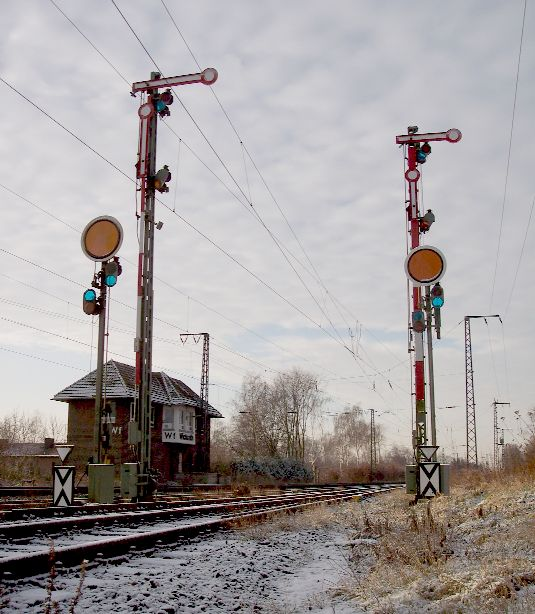
\includegraphics[width=.4\textwidth]{Assets/Images/2-Grundlagen/Formsignale.jpg}
    }}
    \qquad
    \subfloat[\centering Lichtsignal]{{
        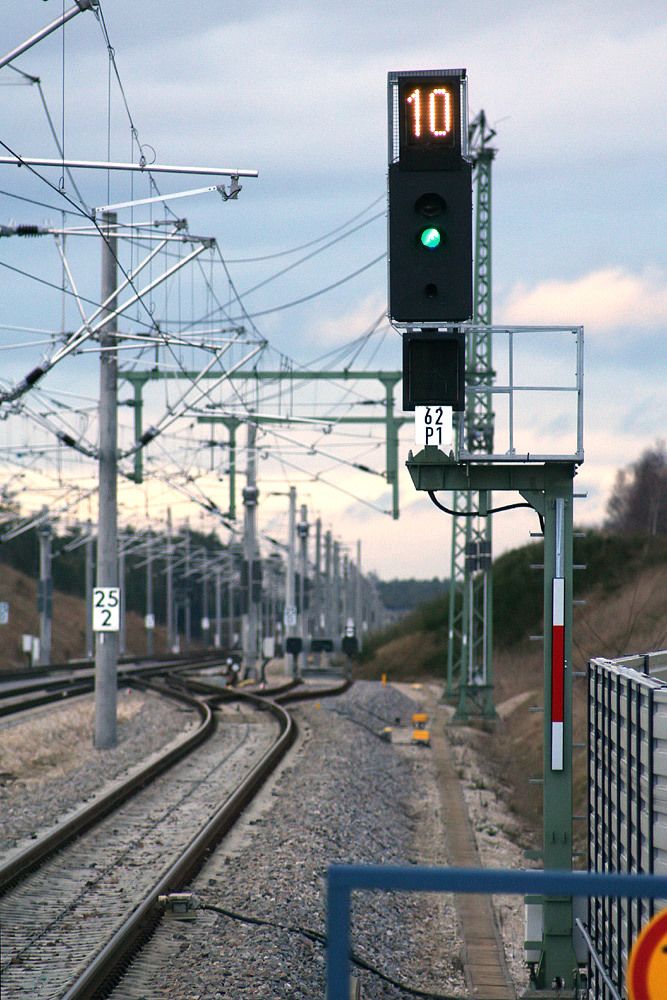
\includegraphics[width=.4\textwidth]{Assets/Images/2-Grundlagen/Ks-Signal.jpg}
    }}
    \caption{Beispiele für deutsche Eisenbahnsignale}\label{abb:Grundlagen:Stellwerkstechnik:Signale}
\end{figure}

In Deutschland sind mehrere Signalsysteme im Einsatz. Ein Signalsystem beschreibt die Bedeutung der Signale und die zugehörigen Signalbilder. Wie Ampeln im Straßenverkehr können Eisenbahnsignale einem Zug die Weiterfahrt erlauben oder verwehren. Außerdem können zulässige Höchstgeschwindigkeiten und die Richtung, in die ein Fahrweg eingestellt ist, angezeigt werden. Da diese Arbeit ihren Fokus nicht auf Signalisierung legt, soll auf dieses Thema nicht weiter eingegangen werden.

\subsubsection*{Weichen}\label{text:Grundlagen:Stellwerkstechnik:Sicherung-des-Schienenverkehrs:Weichen}

Eine Weiche ist ein technisches Mittel, um die Fahrtrichtung eines Zuges zu ändern. Sie besteht aus mehreren Schienen, die beweglich miteinander verbunden sind. Weichen gehören mit zu den wichtigsten Fahrwegelementen, da erst durch sie ein sinnvoller Eisenbahnbetrieb möglich wird. In \autoref{abb:Grundlagen:Stellwerkstechnik:Weichen} ist beispielhaft eine Weiche dargestellt.

% https://de.wikipedia.org/wiki/Datei:Handweiche_Bayreuth_Sankt_Georgen.JPG
\begin{figure}[H]
    \centering
    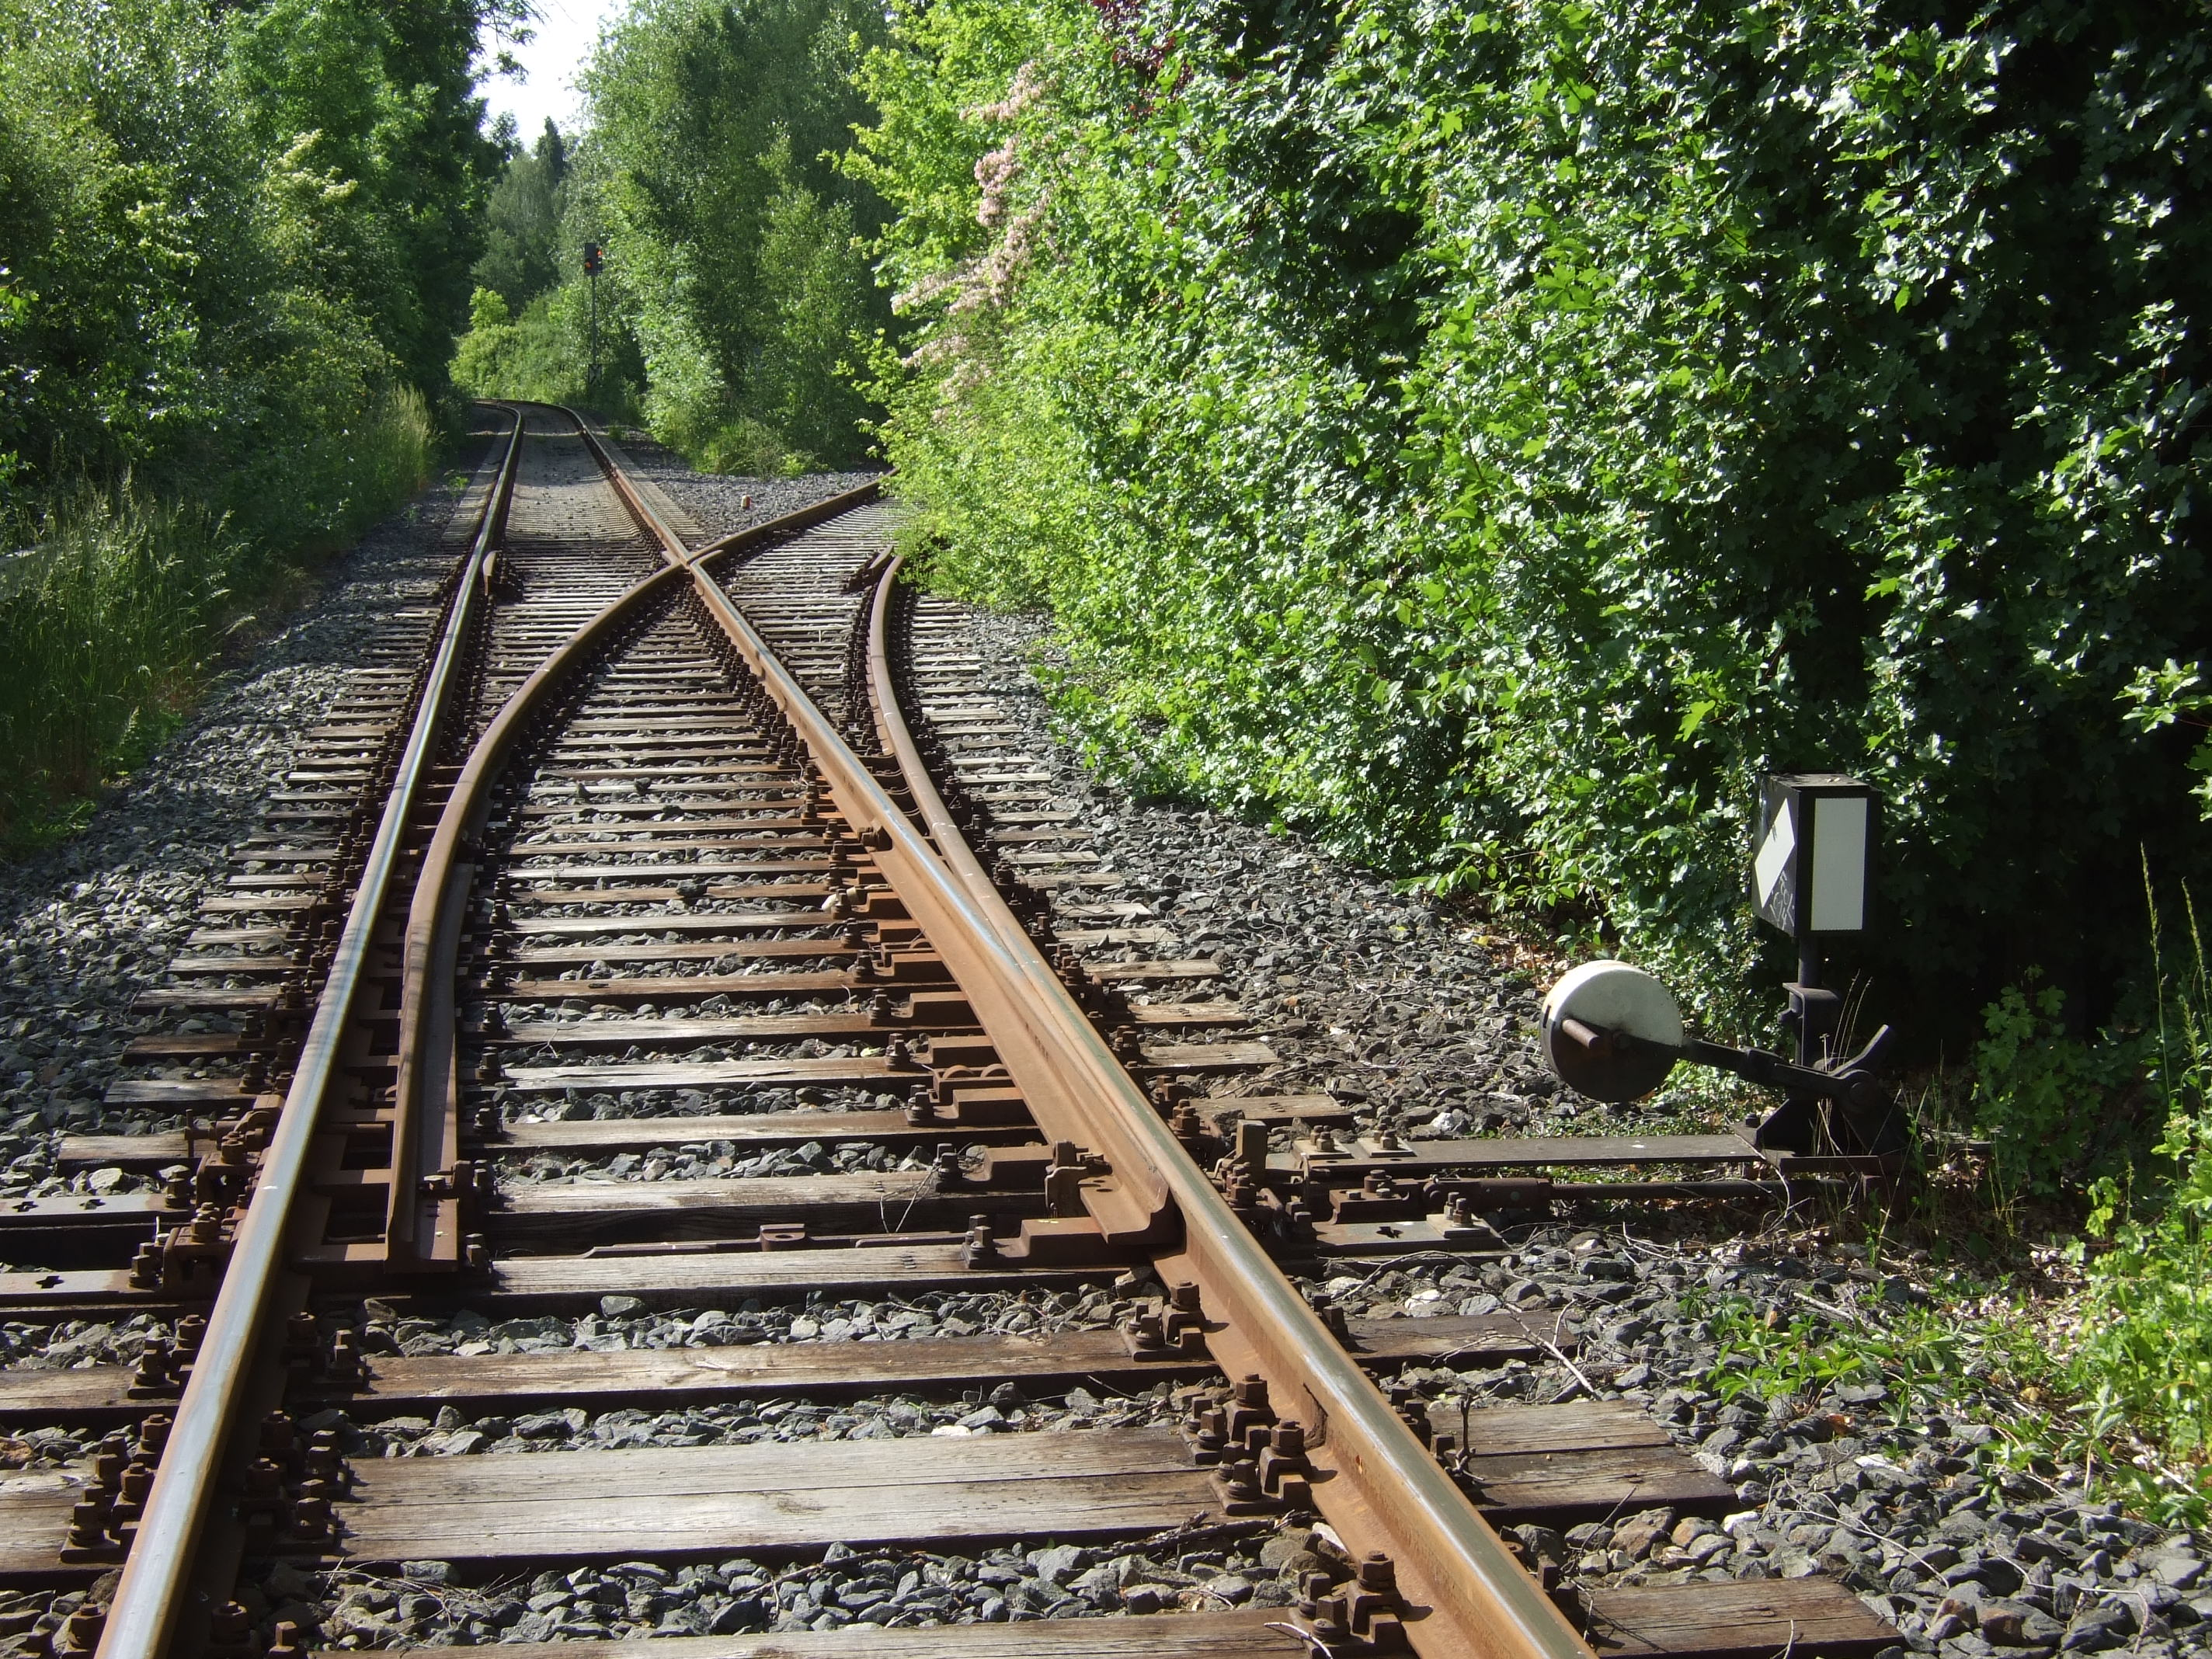
\includegraphics[width=.6\textwidth]{Assets/Images/2-Grundlagen/Handweiche.jpg}
    \caption{Beispiel für eine Weiche}\label{abb:Grundlagen:Stellwerkstechnik:Weichen}
\end{figure}

Weiche gibt es in vielen verschiedenen Ausführungen. Die wichtigste Unterscheidung ist die zwischen \textit{Handweichen} und \textit{elektrischen Weichen}. Handweichen werden von Hand umgestellt. Sie sind die ältere Bauart und werden heute nur noch selten eingesetzt. Elektrische Weichen werden von einem Stellwerk aus umgestellt und sind die heute übliche Bauart. Detaillierter Aufbau und Funktion einer Weiche sind für diese Arbeit nicht relevant. Dennoch soll dieses Thema der Vollständigkeit halber erwähnt werden, da das Konzept der Weiche im weiteren Verlauf dieser Arbeit wieder aufgegriffen wird.

\subsubsection*{Flankenschutz}\label{text:Grundlagen:Stellwerkstechnik:Sicherung-des-Schienenverkehrs:Flankenschutz}

Ein weiteres wichtiges Konzept der Sicherungstechnik ist der Flankenschutz. Er verhindert, dass ein Zug mit einem anderen Zug seitlich kollidiert, also in dessen Flanke fährt. Dies kann insbesondere dann auftreten, falls ein Zug eine ungeplante Fahr- oder Rollbewegung durchführt. Ein Beispiel hierfür ist das zu späte Bremsen bei der Einfahrt in einen Bahnhof. Um Flankenschutz zu gewährleisten, werden Weichen, die gar nicht von einem Zug befahren werden, so gestellt, dass ein auf einem anderen Gleis ungeplant fahrender Zug, nicht in die Flanke des anderen Zuges fahren kann. Um dieses Konzept zu verdeutlichen, sei in \autoref{abb:Grundlagen:Stellwerkstechnik:Flankenschutz} ein beispielhafter, vereinfachter Gleisplan dargestellt.

\todo{Besseres Bild für Flankenschutz finden (selber malen)}
\begin{figure}[H]
    \centering
    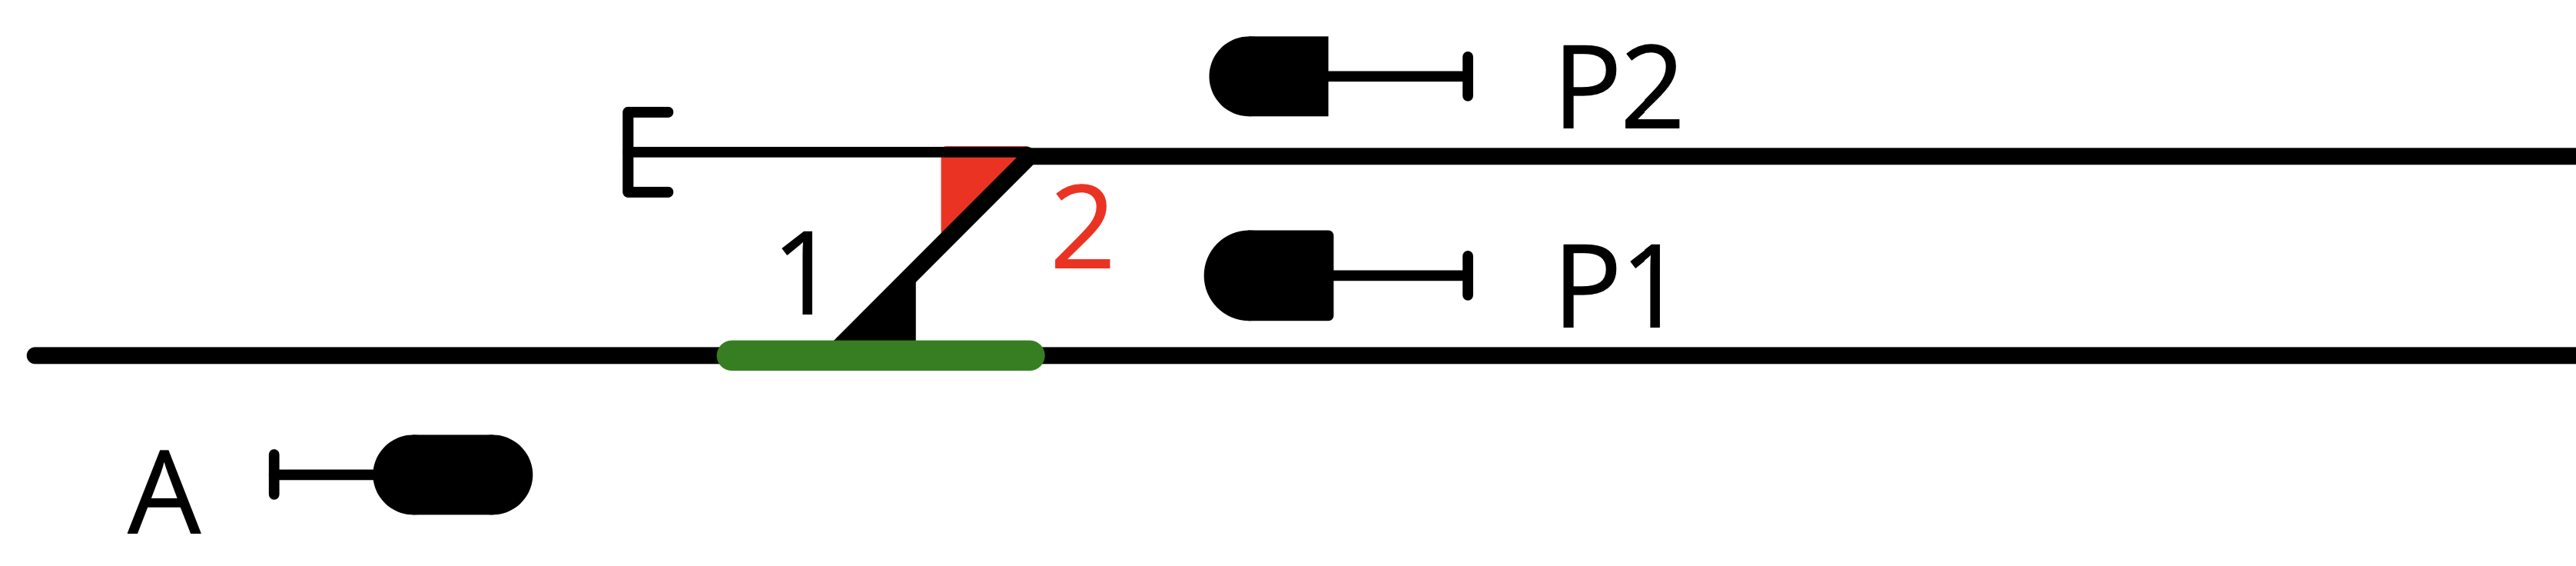
\includegraphics[width=\textwidth]{Assets/Images/2-Grundlagen/Flankenschutz.png}
    \caption{Beispiel für Flankenschutz}\label{abb:Grundlagen:Stellwerkstechnik:Flankenschutz}
\end{figure}

Sei folgendes Szenario gegeben: Es handelt sich um einen Bahnhof mit einem leichten Gefälle nach links. Weiche 2 hat scheinbar keinen Nutzen. Ein Zug steht vor Signal P2. Ein anderer fährt von Signal A nach N1 in den Bahnhof ein. Weiche 1 ist somit in Rechtslage. Jetzt kommt es beim Zug an P2 zu einer ungewollten Lösung der Bremsen und der Zug beginnt zu rollen. Würde Weiche 2 nicht existieren, käme es zu einer Kollision der beiden Züge. Durch Weiche 2 wird der rollende Zug jedoch in ein Stumpfgleis geleitet, wo er zum Stehen kommt. Es kommt zu keiner Kollision. Weiche 2 wird als \textit{Flankenschutzweiche} bezeichnet und hat in diesem einfachen Beispiel auch nur diese eine Funktion. Das Stellwerk stellt sicher, dass der Flankenschutz beim Stellen einer Fahrstraße immer gegeben ist. In der Praxis sind die Gleisanlagen jedoch meist weit umfangreicher und reine Flankenschutzweichen sind selten. Vielmehr sind Flankenschutzweichen Teil von Fahrwegen anderer Züge und nicht immer direkt zu erkennen.

Neben Weichen können auch Signale und andere Fahrwegelemente Flankenschutz bieten. Für diese Arbeit ist jedoch das Verständnis über Flankenschutzweichen ausreichend.

\subsubsection*{Fahrstraße}\label{text:Grundlagen:Stellwerkstechnik:Sicherung-des-Schienenverkehrs:Fahrstrasse}

Der Weg, den ein Zug zurücklegt, setzt sich aus verschiedenen Elementen zusammen:

\begin{itemize}
    \item Gleisabschnitte,
    \item Weichen,
    \item Signale,
    \item weitere Elemente, die hier nicht weiter relevant sind.
\end{itemize}

Die Kombination dieser Elemente wird als \textit{Fahrstraße} bezeichnet. Eine Fahrstraße beginnt und endet in der Regel an einem Signal. Der \ac{Fdl} fordert das Stellwerk zum stellen einer bestimmten Fahrstraße auf, indem er das Start- und Zielsignal eingibt. Aufgabe des Stellwerks ist es nun, einen Fahrweg zwischen den gewünschten Signalen zu finden. Hierbei müssen alle nötigen Fahrwegelemente gefunden und (im Falle von Weichen und Signalen) in die entsprechende Stellung gebracht werden. Wichtig ist hierbei auch das Gewähren von Flankenschutz. Beim Befahren einer Fahrstraße durch einen Zug, werden die Fahrwegelemente nach und nach frei gefahren und können vom Stellwerk wieder für andere Fahrstraßen verwendet werden. Man sagt, die Fahrstraße wird \textit{aufgelöst}.

\subsection{Mechanische Stellwerke}\label{text:Grundlagen:Stellwerkstechnik:Mechanische-Stellwerke}

\subsection{Relaisstellwerke}\label{text:Grundlagen:Stellwerkstechnik:Relaisstellwerke}

\subsection{Elektronische Stellwerke}\label{text:Grundlagen:Stellwerkstechnik:Elektronische-Stellwerke}

\subsection{Digitale Stellwerke}\label{text:Grundlagen:Stellwerkstechnik:Digitale-Stellwerke}

\section{Gleisfreimeldung}\label{text:Grundlagen:Gleisfreimeldung}

Die Gleisfreimeldung ist ein wichtiges Element der Sicherungstechnik im Schienenverkehr. Ihre scheinbar einfache Aufgabe ist es, das Frei- oder Besetztsein eines Gleisabschnittes zu überwachen und dem Stellwerk zu melden. Heutzutage sind zwei verschiedene Arten der Gleisfreimeldung im Einsatz: Gleisstromkreise und Achszähler. In diesem Abschnitt werden nach einer Betrachtung der Historie, beide Systeme vorgestellt und ihre Funktionsweise erläutert.

\subsection{Historische Gleisfreimeldung}\label{text:Grundlagen:Gleisfreimeldung:Historische-Gleisfreimeldung}

\subsection{Gleisstromkreis}\label{text:Grundlagen:Gleisfreimeldung:Gleisstromkreis}

Gleisstromkreise bestimmen den Belegungszustand eines Freimeldeabschnitts über Stromkreise, die durch die Räder der Schienenfahrzeuge geschlossen werden.~\cite[][S. 47]{bib:Sicherung-des-Schienenverkehrs} \autoref{abb:Grundlagen:Gleisfreimeldung:Gleisstromkreis} zeigt den Aufbau eines Gleisstromkreises.

\begin{figure}[H]
    \centering
    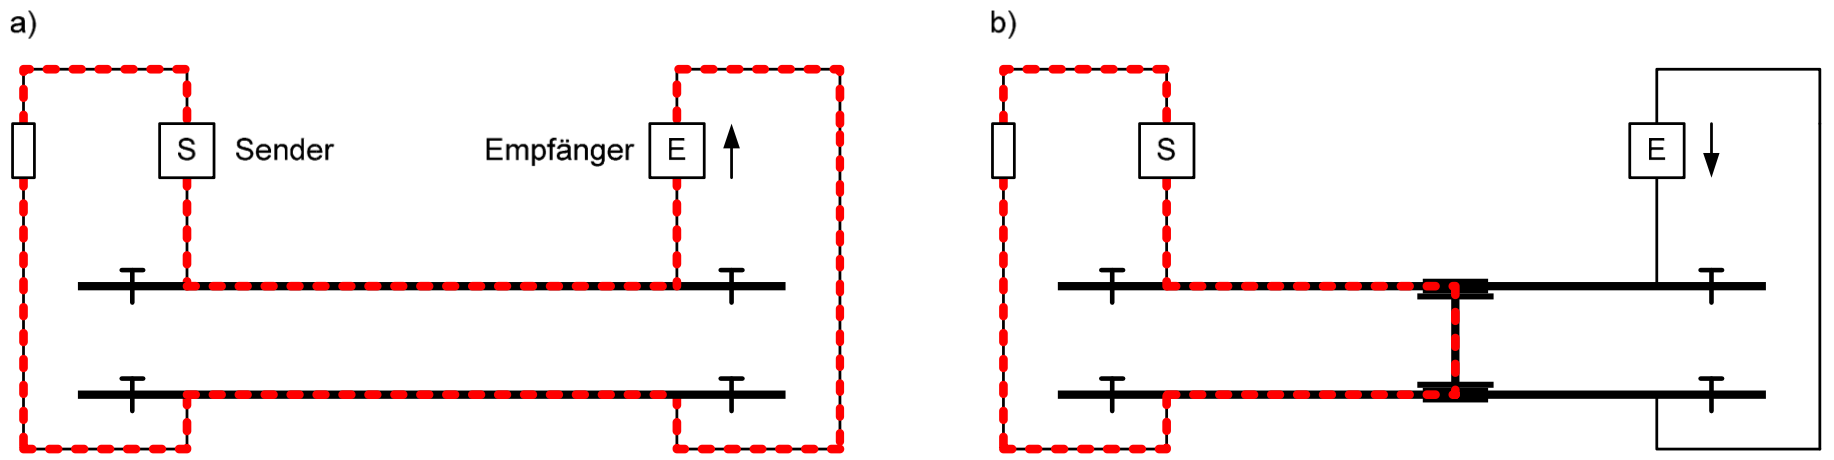
\includegraphics[width=0.7\textwidth]{Assets/Images/2-Grundlagen/Gleisstromkreis.png}
    \caption{Aufbau eines Gleisstromkreises~\cite[][S. 47]{bib:Sicherung-des-Schienenverkehrs}}\label{abb:Grundlagen:Gleisfreimeldung:Gleisstromkreis}
\end{figure}

\textquote{Gleisstromkreise arbeiten nach dem Ruhestromprinzip. Dabei liegt in Grundstellung (freies Gleis) ein geschlossener Stromkreis vor.}~\cite[][S. 47]{bib:Sicherung-des-Schienenverkehrs} Wird ein Gleisabschnitt durch ein Schienenfahrzeug belegt, wird der Stromkreis unterbrochen. Die Unterbrechung des Stromkreises wird vom Stellwerk registriert und als belegt gemeldet.~\cite[][S. 47]{bib:Sicherung-des-Schienenverkehrs} Befindet sich eine Achse im Gleisfreimeldeabschnitt, so wird der Stromkreis geschlossen und der Abschnitt dem Stellwerk besetzt gemeldet.~\cite[][S. 47]{bib:Sicherung-des-Schienenverkehrs}

Ein großer Vorteil von Gleisstromkreisen ist, dass sie in der Lage sind auch stehende Fahrzeuge zu erkennen. Allerdings kann es bei Störungen der Leitfähigkeit der Schienen zu Fehlmeldungen kommen.

\subsection{Achszähler}\label{text:Grundlagen:Gleisfreimeldung:Achszähler}

Achszähler bestimmen den Belegungszustand eines Freimeldeabschnitts über die Zählung der ein- und ausfahrenden Achsen.~\cite[][S. 53]{bib:Sicherung-des-Schienenverkehrs} \autoref{abb:Grundlagen:Gleisfreimeldung:Achszaehlkreis} zeigt den Aufbau eines Achszählkreises.

\begin{figure}[H]
    \centering
    \includegraphics[width=0.7\textwidth]{Assets/Images/2-Grundlagen/Achszählkreis.png}
    \caption{Aufbau eines Achszählkreises~\cite[][S. 53]{bib:Sicherung-des-Schienenverkehrs}}\label{abb:Grundlagen:Gleisfreimeldung:Achszaehlkreis}
\end{figure}

Am Gleis sind Elektromagnete (Schienenkontakte), angebracht, deren Magnetfeld bei Überfahrt eines Rades gestört wird. Diese Störung wird registriert und die Achse gezählt. Achszähler sind in der Lage, die Fahrtrichtung zu bestimmen, indem zwei nah beieinander liegende Schienenkontakte verbaut werden.~\cite[][S. 53 ff.]{bib:Sicherung-des-Schienenverkehrs} \autoref{abb:Grundlagen:Gleisfreimeldung:Doppelter-Schienenkontakt} zeigt einen solchen doppelten Schienenkontakt.

\begin{figure}[H]
    \centering
    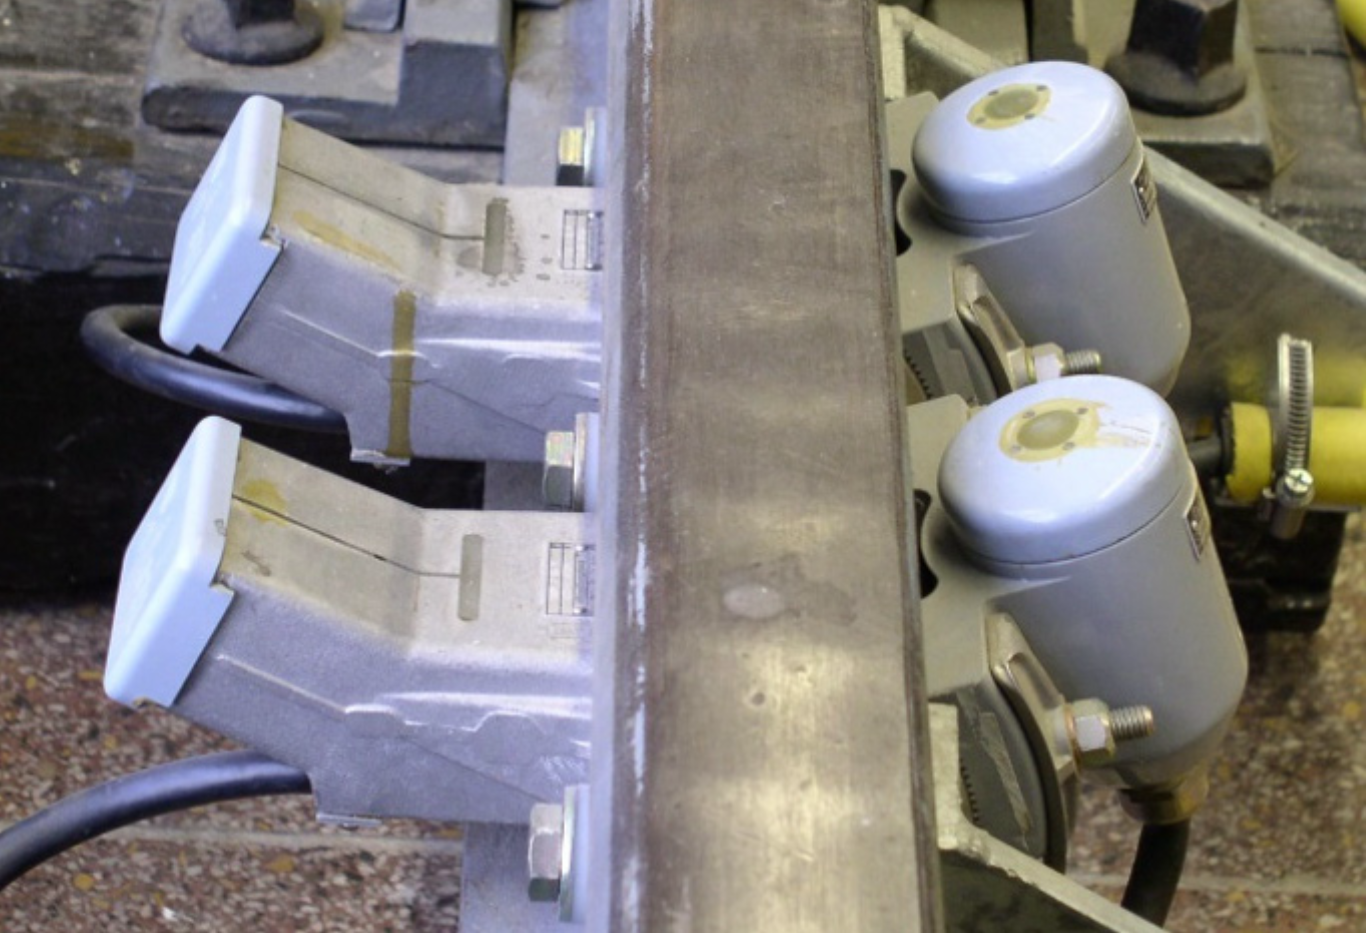
\includegraphics[width=0.7\textwidth]{Assets/Images/2-Grundlagen/Doppelter-Schienenkontakt.png}
    \caption{Doppelter Schienenkontakt~\cite[][S. 54]{bib:Sicherung-des-Schienenverkehrs}}\label{abb:Grundlagen:Gleisfreimeldung:Doppelter-Schienenkontakt}
\end{figure}

Im Gegensatz zu Gleisstromkreisen sind Achszähler nicht in der Lage stehende Fahrzeuge zu erkennen, können jedoch die Fahrtrichtung feststellen.

\section{Steuerung von Modelleisenbahnen}\label{text:Grundlagen:Steuerung-von-Modelleisenbahnen}

Modelleisenbahnen können auf zwei Arten gesteuert werden: analog und digital. In diesem Abschnitt werden beide Methoden vorgestellt.

Nicht relevant für diesen Abschnitt sind weitere Unterscheidungsmerkmale von Modelleisenbahnen, wie die Nenngröße\footnote{Maßstab einer Modelleisenbahn; in Deutschland verbreitete Nenngrößen: H0 und N} oder das Gleissystem (Zweileiter oder Dreileiter).

\subsection{Analoge Steuerung}\label{text:Grundlagen:Steuerung-von-Modelleisenbahnen:Analoge-Steuerung}

Die analoge Steuerung einer Modelleisenbahn ist die älteste und einfachste Methode. Hierbei wird an die isolierten Schienen eines Gleises eine Spannung angelegt --- in der Regel Gleichstrom. Die Lokomotive hat Räder aus Metall, welche die Spannung aufnehmen und direkt an einen Elektromotor weitergeben. Die Geschwindigkeit eines Zuges wird über die Spannung geregelt, dessen Fahrtrichtung über die Polung. Für gewöhnlich hat der Modelleisenbahner einen regelbaren Transformator, mit dem er die Spannung und somit die Geschwindigkeit der Lokomotive steuern kann.~\cite[][S. 178 ff.]{bib:Modellbauhandbuch}

In \autoref{abb:Grundlagen:Steuerung-von-Modelleisenbahnen:Analoge-Steuerung:Einfaches-Gleisoval} ist ein einfaches Gleisoval dargestellt. An die Gleise ist ein regelbarer Trafo angeschlossen.

\begin{figure}[H]
    \centering
    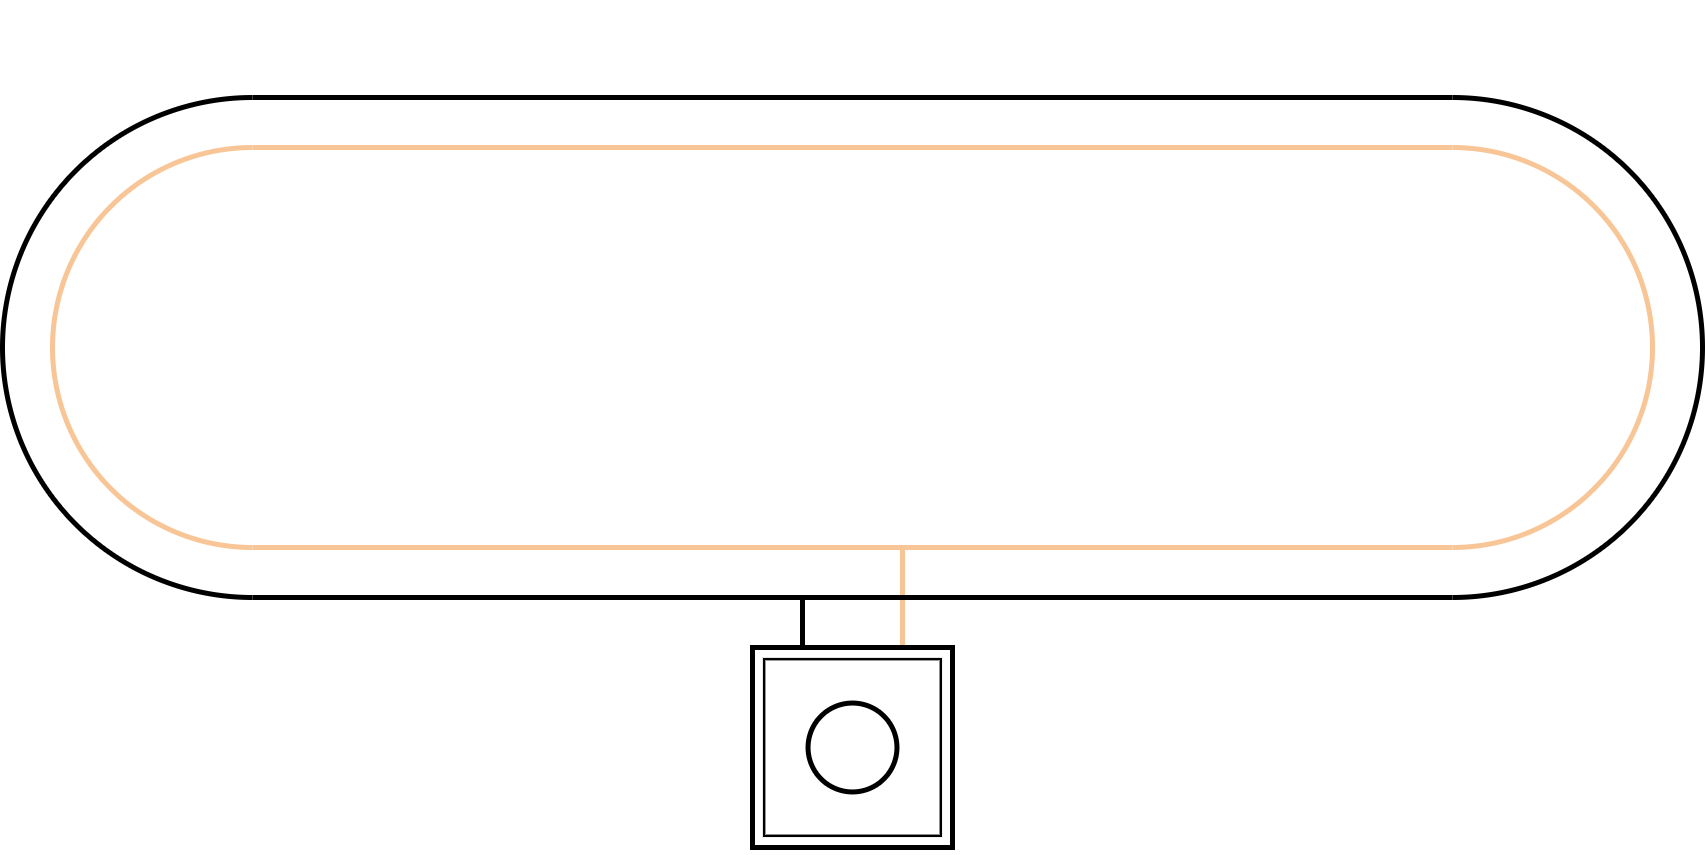
\includegraphics[width=\textwidth]{Assets/Images/2-Grundlagen/Modelleisenbahnen-Einfaches-Gleisoval.png}
    \caption{Einfaches Gleisoval mit regelbarem Trafo~\cite[nach][S. 180]{bib:Modellbauhandbuch}}\label{abb:Grundlagen:Steuerung-von-Modelleisenbahnen:Analoge-Steuerung:Einfaches-Gleisoval}
\end{figure}

Werden nun mehr als ein Zug auf das Gleisoval gesetzt, hat dies zur Folge, dass alle Züge gleichzeitig fahren. Sollen Züge unabhängig voneinander gesteuert werden, so muss das Gleisoval in mehrere Abschnitte unterteilt werden. Dafür werden die Gleise galvanisch getrennt und an die Abschnitte jeweils ein eigener Trafo angeschlossen.~\cite[][S. 181]{bib:Modellbauhandbuch} Bei anspruchsvolleren Anlagen, ist zusätzlich die Nutzung von Polwendeschaltern notwendig, um beispielsweise Gleisschleifen oder Gleisdreiecke zu ermöglichen.~\cite[][S. 183 f.]{bib:Modellbauhandbuch} Eine weitere Möglichkeit ist der Einbau von Schaltern, um bestimmte Gleisabschnitte vom Strom zu trennen.~\cite[][S. 182]{bib:Modellbauhandbuch}

Weichen werden auf einer analogen Modelleisenbahn wahlweise elektrisch oder manuell gestellt. Hierbei ist es der Kreativität des Modellbauers überlassen, wie er die Ansteuerung konkret umsetzt. Der Bau von Schaltbrettern, auf denen alle Weichen kompakt zusammengefasst sind, ist üblich.~\cite[][S. 185]{bib:Modellbauhandbuch} Dasselbe gilt für Signale, sofern man sich auf einer analogen Anlage für deren Einbau entscheidet.
\subsection{Digitale Steuerung}\label{text:Grundlagen:Steuerung-von-Modelleisenbahnen:Digitale-Steuerung}

Eine digitale Modelleisenbahn verfolgt ein grundlegend anderes Konzept. An den Gleisen liegt die ganze Zeit über eine konstante Spannung an. Die Lokomotiven leiten den Strom nicht mehr direkt an den Motor weiter, sondern sind mit einem Decoder ausgestattet. Dieser Decoder ist in der Lage, digitale Signale zu empfangen und in Steuerbefehle umzusetzen. Die Steuerbefehle werden über die Schienen an die Lokomotiven gesendet.

Die digitale Steuerung bietet gegenüber der analogen Steuerung einige Vorteile. So können mehrere Züge unabhängig voneinander gesteuert werden, ohne dass das Gleis in galvanisch getrennte Abschnitte unterteilt werden muss. Optional können Weichen und Signale ebenfalls digital gesteuert werden.

Durch den Einsatz digital gesteuerter Züge und Weichen ist eine Steuerung durch einen Computer möglich. Die gängigen Programme erlauben es, den Gleisplan schematisch nachzubauen und die gesamte Anlage per Mausklick zu steuern. Eine Vollautomatisierung der Anlage, wie es beispielsweise bei großen Anlagen zwingend notwendig ist, kann ebenfalls realisiert werden.

Für einen automatischen Betrieb der Anlage ist auch bei einer Modelleisenbahn eine Gleisfreimeldeanlage notwendig. Man spricht hier in der Regel von Rückmeldern. Realisiert werden sie über die Unterteilung der Strecke in Einspeiseabschnitte, die mit einem Rückmeldemodul verbunden sind. Fährt ein Zug in einen neuen Abschnitt ein, wird der Strom aus diesem Abschnitt gezogen und die neue Position ist somit bekannt. Hierfür ist eine präzise Konfiguration notwendig, da die Länge eines Zuges bekannt sein muss. Die exakte Position kann dann abgeschätzt werden.


\chapter{Methodik}\label{text:Methodik}

Bei der Automatisierung einer Modelleisenbahn eröffnet sich ein breites Spektrum an Entscheidungsmöglichkeiten, die durch verschiedene Ansätze und Technologien realisiert werden können. Jeder dieser Entscheidungspunkte birgt das Potential, Effizienz, Realitätsnähe und den Unterhaltungswert der Modelleisenbahn wesentlich zu verändern. In diese Kapitel werden verschiedene Methoden und Technologien vorgestellt, die für die Umsetzung der Automatisierung einer Modelleisenbahn in Frage kommen. Es werden spezifische Kriterien und Überlegungen beleuchtet, die bei der Auswahl der geeigneten Umsetzungsmethode berücksichtigt werden müssen. Das Ziel besteht darin, ein tiefgreifendes Verständnis dafür zu entwickeln, wie jede Entscheidung die Konzeption und Funktionalität der automatisierten Modelleisenbahn beeinflusst.

\newpage
\input{Text/3-Methodik/Achszähler.tex}
\newpage
\section{Systemkonfiguration}\label{text:Methodik:Systemkonfiguration}

Die Automatisierung einer Modelleisenbahn stellt ein faszinierendes Unterfangen dar, das eine Brücke zwischen technischer Innovation und nostalgischer Leidenschaft schlägt. Die Auswahl der geeigneten Technik zur Realisierung dieses Ziels erfordert eine gründliche Überlegung verschiedener Ansätze. Dieser Abschnitt widmet sich der Vorstellung von zwei maßgeblichen Varianten, die für die Implementierung des Projekts in Erwägung gezogen werden. Dabei werden nicht nur die technischen Aspekte beleuchtet, sondern auch die praktischen Auswirkungen jeder Variante auf das Gesamtprojekt diskutiert.

\subsection{Zentrale Steuerung}\label{text:Methodik:Systemkonfiguration:Zentrale-Steuerung}

Die Idee einer zentralen Steuerung ist in der Welt der Automatisierung keineswegs neu, findet aber in der Konzeption von Modelleisenbahnsystemen eine besondere Anwendung. Kern dieses Ansatzes ist es, sämtliche Komponenten - von den Weichen über die Signale bis hin zu den Achszählern - unter der Ägide einer zentralen Steuereinheit zu vereinen. Ein Raspberry Pi, bekannt für seine Vielseitigkeit und Leistungsfähigkeit, erweist sich als ideale Wahl für eine solche Steuereinheit. Seine Fähigkeit, zahlreiche Sensoren und Aktuatoren über GPIO-Pins anzusteuern, ermöglicht eine nahtlose Integration und Kontrolle der verschiedenen Systemelemente.
\newline
Ein bedeutender Aspekt der zentralen Steuerung ist die Kommunikation mit dem Benutzer. Der Raspberry Pi kann über eine grafische Benutzeroberfläche (GUI) verfügen, die es dem Benutzer ermöglicht, die Modelleisenbahn zu steuern und zu überwachen. Die GUI kann beispielsweise die Position der Züge auf der Anlage anzeigen, die Weichen und Signale steuern und die Achszähler überwachen. Die zentrale Steuerung bietet somit eine umfassende Kontrolle über die Modelleisenbahn und ermöglicht eine intuitive Interaktion mit dem System.

\subsection{Dezentrale Steuerung}\label{text:Methodik:Systemkonfiguration:Dezentrale-Steuerung}

Während die zentrale Steuerung durch ihre Einheitlichkeit besticht, bietet die dezentrale Steuerung eine Flexibilität, die in komplexen oder sich erweiternden Systemen von unschätzbarem Wert sein kann. Hierbei werden die Achszähler und weitere Systemkomponenten als autonome Einheiten konzipiert, die über individuelle Mikrocontroller gesteuert werden. Diese Mikrocontroller, beispielsweise aus der Arduino- oder ESP-Familie, sind dafür verantwortlich, ihre jeweiligen Bereiche autonom zu verwalten und dabei dennoch eine übergeordnete Koordination durch einen zentralen Computer - das virtuelle Stellwerk - zu ermöglichen.
\newline
Diese Methode brilliert durch ihre modulare Natur. Jede Komponente kann unabhängig entwickelt, getestet und bei Bedarf ersetzt oder erweitert werden. Darüber hinaus erlaubt die dezentrale Architektur eine skalierbare Erweiterung der Anlage, ohne dass die Grundstruktur des Systems grundlegend überdacht werden muss. Allerdings erfordert dieser Ansatz eine sorgfältige Planung der Kommunikationswege zwischen den Mikrocontrollern und dem zentralen Stellwerk, um Effizienz und Zuverlässigkeit zu gewährleisten.

\subsection{Entscheidung}\label{text:Methodik:Systemkonfiguration:Entscheidung}

Nach eingehender Betrachtung der Vor- und Nachteile beider Systeme fiel die Entscheidung auf eine innovative Hybridlösung, die die Stärken beider Ansätze vereint. Diese Lösung sieht vor, dass Achszähler, Weichen und Signale dezentral über Mikrocontroller gesteuert werden, wobei mehrere Sensoren und Aktuatoren an einen einzigen Controller angeschlossen werden können. Ein Beispiel hierfür ist die Nutzung eines Raspberry Pi Pico, der mehrere Achszähler steuert und somit die Effizienz des Systems steigert.
\newline
Die zentrale Steuerung des Stellwerks erfolgt durch ein speziell entwickeltes Programm auf einem Laptop, der eine direkte Verbindung zu den Mikrocontrollern unterhält. Diese Konfiguration optimiert die Flexibilität und Modularität der Anlage und ermöglicht gleichzeitig eine zentrale Überwachung und Steuerung. Durch die Kombination der Sensoren und Aktuatoren an einzelnen Mikrocontrollern können die Kosten effektiv gesenkt werden, während die Modularität und Erweiterbarkeit des Systems erhalten bleiben.
\newline
Die Entscheidung für diese Hybridlösung spiegelt das Bestreben wider, eine Balance zwischen technischer Effizienz, Kostenkontrolle und der Realisierung einer realitätsnahen Modelleisenbahn zu finden. Sie symbolisiert einen innovativen Ansatz in der Welt der Modelleisenbahnautomatisierung, der die Grundlage für zukünftige Entwicklungen und Erweiterungen bildet.
\newline
Die Kommunikation zwischen den Mikrocontrollern untereinander und dem Laptop wird in \autoref{text:Methodik:Kommunikation} näher erläutert.

\newpage
\section{Kommunikation}\label{text:Methodik:Kommunikation}

Die effiziente und zuverlässige Kommunikation zwischen dem Laptop, der als Steuerzentrale dient, und den Mikrocontrollern, welche die Achszähler steuern, ist ein fundamentales Element für die Funktionalität des gesamten Systems. Hierbei kommen verschiedene Schnittstellen und Protokolle in Frage, um eine reibungslose und effektive Übertragung von Steuerbefehlen und Zustandsinformationen zu gewährleisten. Im Folgenden werden die charakteristischen Merkmale und Implementierungsdetails der verschiedenen Kommunikationsmöglichkeiten erörtert, wobei auch auf deren Eignung für spezifische Anwendungsfälle eingegangen wird.

\subsection{CAN-Bus}\label{text:Methodik:Kommunikation:CAN-Bus}

Der CAN-Bus, ein für die Automobilbranche konzipiertes serielles Bussystem, ermöglicht eine effiziente Kommunikation zwischen den diversen Steuergeräten innerhalb eines Fahrzeugs. Als Zweidrahtsystem konstruiert, basiert es auf einem High- und einem Low-Pin für den Datenaustausch. Diese Architektur gewährleistet eine robuste Vernetzung der Steuergeräte, wodurch sie Informationen teilen und aufeinander abstimmen können. Hervorzuheben ist die ausgeprägte Fehlertoleranz des Systems sowie seine Fähigkeit, hohe Datenübertragungsraten zu unterstützen. Neben seiner Anwendung in Fahrzeugen eignet sich der CAN-Bus auch hervorragend für Modelleisenbahnen, dank seiner hohen Leistungsfähigkeit und Zuverlässigkeit. Ein CAN-Bus zwischen mehreren Raspberry Pi Pico Mikrocontrollern kann wie folgt realisiert werden:

\begin{figure}[H]
    \centering
    \includegraphics[width=0.7\textwidth]{Assets/Images/3-Methodik/CANBus-Test.png}
    \caption{CAN-Bus zwischen mehreren Raspberry Pi Pico Mikrocontrollern}\label{fig:Methodik:Kommunikation:CAN-Bus}
\end{figure}

In \autoref{fig:Methodik:Kommunikation:CAN-Bus} ist ein CAN-Bus zwischen zwei Raspberry Pi Pico Mikrocontrollern dargestellt. Der CAN-Bus besteht aus einem Kreis, welcher mit 120 Ohm Widerständen an beiden Enden abgeschlossen ist. Die beiden Mikrocontroller sind über den CAN-Bus miteinander verbunden und können so miteinander kommunizieren. Die Kommunikation erfolgt über die Pins GPIO0 und GPIO1 beider Controller. Die Kommunikation zwischen den Mikrocontrollern wird mit der \lstinline{can2040} \footnote{\url{https://github.com/KevinOConnor/can2040}} Bibliothek realisiert. Diese Bibliothek ermöglicht die Kommunikation über den CAN-Bus und bietet eine einfache API, um Nachrichten zu senden und zu empfangen. Die LEDs auf dem Breadboard veranschaulichen das Ping-Pong-Programm, welches die Kommunikation zwischen den beiden Mikrocontrollern darstellt. Der Mikrocontroller 1 sendet eine Nachricht an den Mikrocontroller 2, welcher diese Nachricht empfängt und eine Antwort zurücksendet. Der Mikrocontroller 1 empfängt diese Antwort und sendet wieder eine Nachricht an den Mikrocontroller 2. Dieser Vorgang wiederholt sich in einer Endlosschleife.

\subsection{UART}\label{text:Methodik:Kommunikation:UART}

UART (Universal Asynchronous Receiver Transmitter) ist ein asynchrones seriell arbeitendes Kommunikationsprotokoll, das in der Regel für die Kommunikation zwischen Mikrocontrollern und anderen Geräten verwendet wird. Es ermöglicht die Übertragung von Daten zwischen zwei Geräten über eine einzige Datenleitung. Die Kommunikation erfolgt über die Pins TX und RX beider Geräte.
\newline
Der Raspberry Pi Pico verfügt über zwei UART-Ports. Mithilfe dieser Ports kann ein Bus zwischen mehreren Mikrocontrollern realisiert werden, welcher quasi unendlich erweiterbar ist. Die Kommunikation zwischen den Mikrocontrollern mittels UART ist bereits in der pico-sdk Bibliothek implementiert.

\subsection{Analoge Kommunikation}\label{text:Methodik:Kommunikation:Analoge-Kommunikation}

Die Kommunikation zwischen den Mikrocontrollern kann auch über analoge Signale realisiert werden. Hierbei wird ein Signal von einem Mikrocontroller erzeugt und an den anderen Mikrocontroller übertragen. Dieser Mikrocontroller empfängt das Signal und kann daraufhin eine Aktion ausführen. Die Kommunikation erfolgt über die Pins eines Mikrocontrollers. Die Kommunikation mittels analoger Signale ist jedoch sehr langsam und unzuverlässig. Deshalb wird diese Methode nicht weiter betrachtet.

\subsection{Anmerkung}\label{text:Methodik:Kommunikation:Anmerkung}

Die Verbindung zwischen dem Steuerlaptop und den Mikrocontrollern über die USB-Schnittstelle stellt eine zentrale Komponente des Kommunikationssystems dar. Ein Raspberry Pi Pico agiert hierbei als Brücke, indem er als USB-zu-Bus-Interface fungiert. Die \lstinline{tinyusb} \footnote{\url{https://github.com/hathach/tinyusb}} Bibliothek ermöglicht eine effiziente und flexible Kommunikation über diese Schnittstelle, wodurch eine hohe Kompatibilität und einfache Integration in das Gesamtsystem gewährleistet wird. 


\chapter{Entwicklung der Gleisfreimeldeanlage}\label{text:Entwicklung-der-GFA}

In den vorangegangen Kapiteln wurde beschrieben, wie die Stellwerkstechnik bei realen Eisenbahnen funktioniert und mögliche Umsetzungen für die Automatisierung einer Modelleisenbahn vorgestellt. In diesem Kapitel soll die Entwicklung der Gleisfreimeldeanlage beschrieben werden.

\input{Text/4-Entwicklung-der-GFA/Achszähler.tex}
\newpage
\section{Gleisfreimeldung}\label{text:Grundlagen:Gleisfreimeldung}

Die Gleisfreimeldung ist ein wichtiges Element der Sicherungstechnik im Schienenverkehr. Ihre scheinbar einfache Aufgabe ist es, das Frei- oder Besetztsein eines Gleisabschnittes zu überwachen und dem Stellwerk zu melden. Heutzutage sind zwei verschiedene Arten der Gleisfreimeldung im Einsatz: Gleisstromkreise und Achszähler. In diesem Abschnitt werden nach einer Betrachtung der Historie, beide Systeme vorgestellt und ihre Funktionsweise erläutert.

\subsection{Historische Gleisfreimeldung}\label{text:Grundlagen:Gleisfreimeldung:Historische-Gleisfreimeldung}

\subsection{Gleisstromkreis}\label{text:Grundlagen:Gleisfreimeldung:Gleisstromkreis}

Gleisstromkreise bestimmen den Belegungszustand eines Freimeldeabschnitts über Stromkreise, die durch die Räder der Schienenfahrzeuge geschlossen werden.~\cite[][S. 47]{bib:Sicherung-des-Schienenverkehrs} \autoref{abb:Grundlagen:Gleisfreimeldung:Gleisstromkreis} zeigt den Aufbau eines Gleisstromkreises.

\begin{figure}[H]
    \centering
    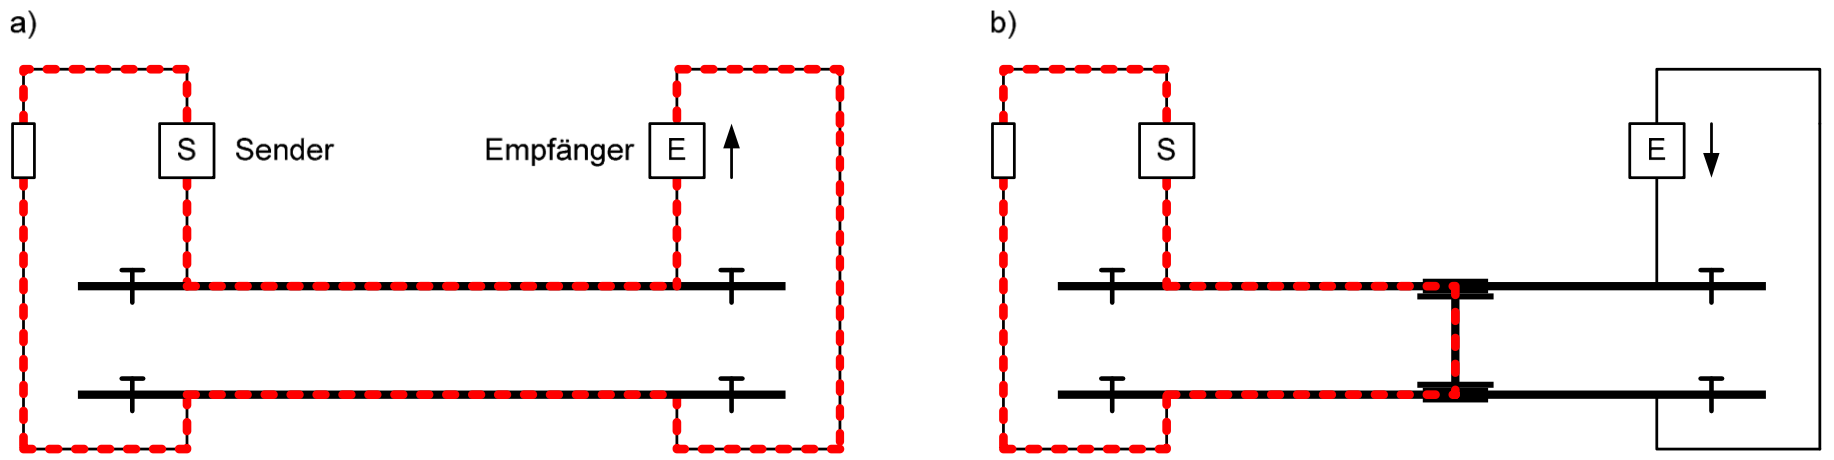
\includegraphics[width=0.7\textwidth]{Assets/Images/2-Grundlagen/Gleisstromkreis.png}
    \caption{Aufbau eines Gleisstromkreises~\cite[][S. 47]{bib:Sicherung-des-Schienenverkehrs}}\label{abb:Grundlagen:Gleisfreimeldung:Gleisstromkreis}
\end{figure}

\textquote{Gleisstromkreise arbeiten nach dem Ruhestromprinzip. Dabei liegt in Grundstellung (freies Gleis) ein geschlossener Stromkreis vor.}~\cite[][S. 47]{bib:Sicherung-des-Schienenverkehrs} Wird ein Gleisabschnitt durch ein Schienenfahrzeug belegt, wird der Stromkreis unterbrochen. Die Unterbrechung des Stromkreises wird vom Stellwerk registriert und als belegt gemeldet.~\cite[][S. 47]{bib:Sicherung-des-Schienenverkehrs} Befindet sich eine Achse im Gleisfreimeldeabschnitt, so wird der Stromkreis geschlossen und der Abschnitt dem Stellwerk besetzt gemeldet.~\cite[][S. 47]{bib:Sicherung-des-Schienenverkehrs}

Ein großer Vorteil von Gleisstromkreisen ist, dass sie in der Lage sind auch stehende Fahrzeuge zu erkennen. Allerdings kann es bei Störungen der Leitfähigkeit der Schienen zu Fehlmeldungen kommen.

\subsection{Achszähler}\label{text:Grundlagen:Gleisfreimeldung:Achszähler}

Achszähler bestimmen den Belegungszustand eines Freimeldeabschnitts über die Zählung der ein- und ausfahrenden Achsen.~\cite[][S. 53]{bib:Sicherung-des-Schienenverkehrs} \autoref{abb:Grundlagen:Gleisfreimeldung:Achszaehlkreis} zeigt den Aufbau eines Achszählkreises.

\begin{figure}[H]
    \centering
    \includegraphics[width=0.7\textwidth]{Assets/Images/2-Grundlagen/Achszählkreis.png}
    \caption{Aufbau eines Achszählkreises~\cite[][S. 53]{bib:Sicherung-des-Schienenverkehrs}}\label{abb:Grundlagen:Gleisfreimeldung:Achszaehlkreis}
\end{figure}

Am Gleis sind Elektromagnete (Schienenkontakte), angebracht, deren Magnetfeld bei Überfahrt eines Rades gestört wird. Diese Störung wird registriert und die Achse gezählt. Achszähler sind in der Lage, die Fahrtrichtung zu bestimmen, indem zwei nah beieinander liegende Schienenkontakte verbaut werden.~\cite[][S. 53 ff.]{bib:Sicherung-des-Schienenverkehrs} \autoref{abb:Grundlagen:Gleisfreimeldung:Doppelter-Schienenkontakt} zeigt einen solchen doppelten Schienenkontakt.

\begin{figure}[H]
    \centering
    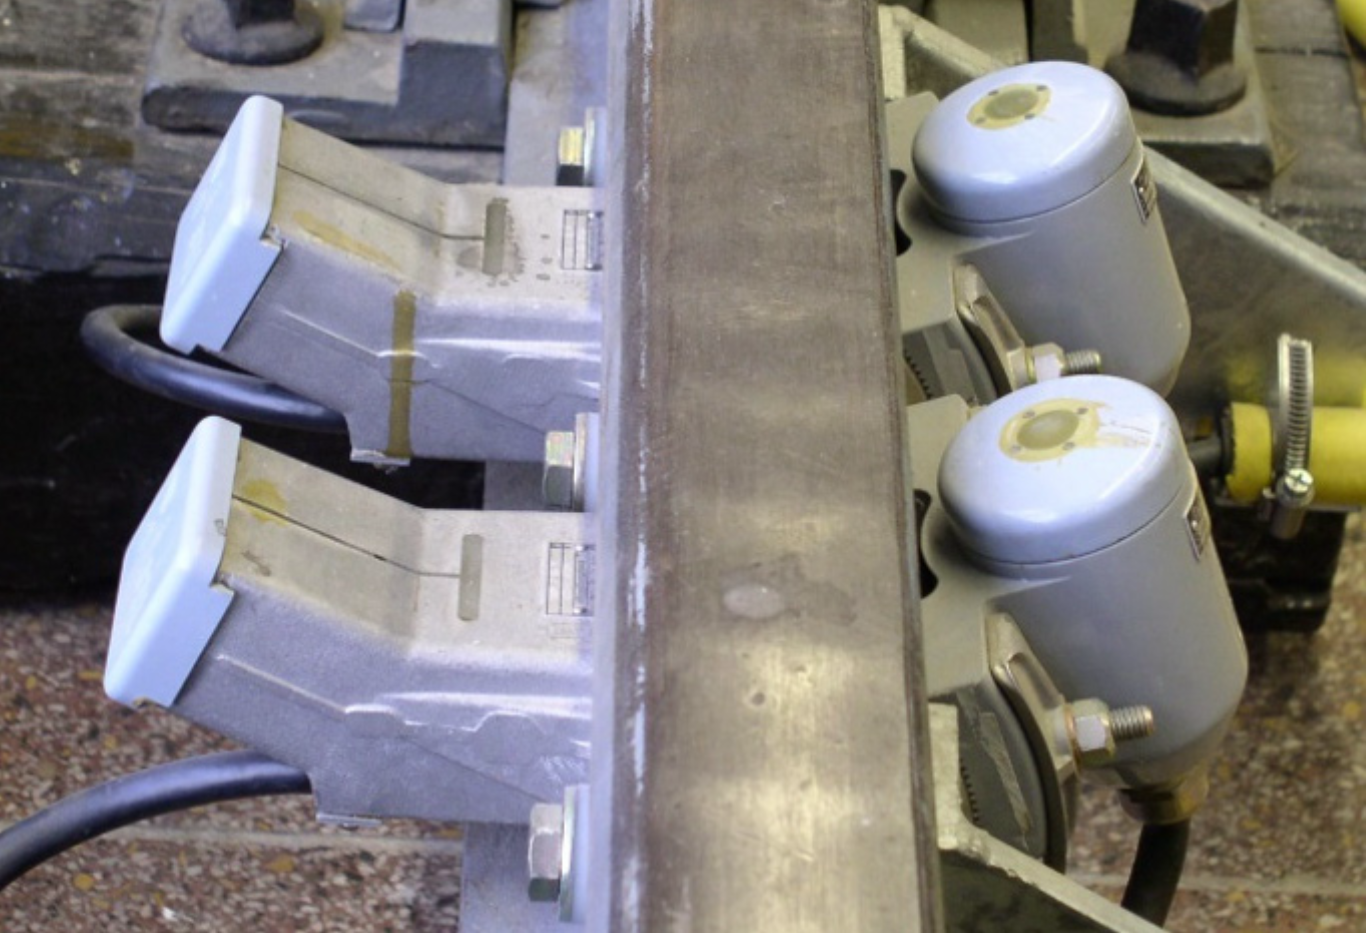
\includegraphics[width=0.7\textwidth]{Assets/Images/2-Grundlagen/Doppelter-Schienenkontakt.png}
    \caption{Doppelter Schienenkontakt~\cite[][S. 54]{bib:Sicherung-des-Schienenverkehrs}}\label{abb:Grundlagen:Gleisfreimeldung:Doppelter-Schienenkontakt}
\end{figure}

Im Gegensatz zu Gleisstromkreisen sind Achszähler nicht in der Lage stehende Fahrzeuge zu erkennen, können jedoch die Fahrtrichtung feststellen.

\newpage
\section{Softwaretests}\label{text:Entwicklung-der-GFA:Softwaretests}

Die Softwaretests sind ein wichtiger Bestandteil der Softwareentwicklung. Sie dienen dazu, die Funktionalität der Software zu überprüfen und Fehler zu finden. In diesem Abschnitt werden die Softwaretests für die Gleisfreimeldeanlage beschrieben.\newline
Die Tests für die Gleisfreimeldeanlage sind Software-seitig in zwei Kategorien unterteilt:
\begin{itemize}
    \item Tests für Geraden
    \item Tests für Weichen
\end{itemize}
Die Test-Skripte wurden nach und nach entwickelt und immer wieder ausgeführt. Somit wurden zunächst die Methoden zur Initialisierung der einzelnen Komponenten getestet und später die Methoden zur Überprüfung der Funktionalität der Gleisfreimeldeanlage.

\subsection{Tests für Geraden}\label{text:Entwicklung-der-GFA:Softwaretests:Tests-für-Geraden}

Das Testprogramm startet mit der Initialisierung der einzelnen Komponenten. Da das Skript zu lange ist um es hier komplett darzustellen, wird nur ein Ausschnitt dessen gezeigt. Für das Verständnis ist es wichtig die folgenden Definitionen zu kennen:
\begin{itemize}
    \item p1, p2, p3, p4 sind Kontaktpunkte
    \item d1 ist ein gerichteter Achszähler, der die Kontaktpunkte p1 und p2 verwendet
    \item d2 ist ein gerichteter Achszähler, der die Kontaktpunkte p3 und p4 verwendet
    \item c ist ein Counter/ Streckenabschnitt
    \item v ist die Gleisfreimeldeanlage
\end{itemize}


\newpage
\chapter{Entwicklung des Stellwerks}\label{text:Entwicklung-des-Stellwerks}

In den vorangegangen Kapiteln wurde beschrieben, wie die Stellwerkstechnik bei realen Eisenbahnen funktioniert. Das Wissen über Gleisfreimeldeanlagen wurde auf den Kontext einer Klemmbausteineisenbahn übertragen und eine für diesen Zweck geeignete Gleisfreimeldeanlage entwickelt. In diesem Kapitel soll die Entwicklung des Stellwerks beschrieben werden.

Hierfür wird in \autoref{text:Entwicklung-des-Stellwerks:Fahrstrassenlogik} \nameref{text:Entwicklung-des-Stellwerks:Fahrstrassenlogik} auf den Kern des Stellwerks eingegangen, die Bildung und Auflösung von Fahrstraßen. Anschließend erläutert \autoref{text:Entwicklung-des-Stellwerks:Gleisfreimeldeanlage} \nameref{text:Entwicklung-des-Stellwerks:Gleisfreimeldeanlage} die Implementierung der Gleisfreimeldeanlage. Danach wird in \autoref{text:Entwicklung-des-Stellwerks:Signaldecoder} \nameref{text:Entwicklung-des-Stellwerks:Signaldecoder} und \autoref{text:Entwicklung-des-Stellwerks:Weichendecoder} \nameref{text:Entwicklung-des-Stellwerks:Weichendecoder} auf die Ansteuerung der Signale und die Ansteuerung der Weichen eingegangen. Abschließend zeigt \autoref{text:Entwicklung-des-Stellwerks:Bedienung} \nameref{text:Entwicklung-des-Stellwerks:Bedienung} wie das Stellwerk zu bedienen ist.

Das gesamte Kapitel bezieht sich im speziellen auf den in \autoref{abb:Entwicklung-des-Stellwerks:Bahnhof-Gleisplan} dargestellten Gleisplan. Eine umfangreichere Gleisanlage wäre wünschenswert gewesen, war aber aufgrund mangelnden Materials nicht möglich.

\begin{figure}[H]
    \centering
    
\includegraphics[width=\textwidth]{Assets/Images/5-Entwicklung-des-Stellwerks/Bahnhof-Gleisplan.png}
    \caption{Gleisplan des Bahnhofs}\label{abb:Entwicklung-des-Stellwerks:Bahnhof-Gleisplan}
\end{figure}

Der Bahnhof und alle anderen Elemente wurden mit Steinen des dänischen Klemmbausteinherstellers LEGO\textsuperscript{\tiny{\textregistered}} gebaut.

An dieser Stelle muss erwähnt werden, dass bei der Entwicklung des Stellwerks große Probleme auftraten. Während die Entwicklung der Fahrstraßenlogik und der Gleisfreimeldeanlage weitestgehend reibungslos vonstatten ging, gelang es nicht, die einzelnen Komponenten kommunizieren zu lassen. Daher wurden der Signaldecoder und der Weichendecoder nicht implementiert und können nur konzeptuell behandelt werden. Eine detailliertere Problembeschreibung findet sich in \autoref{text:Entwicklung-des-Stellwerks:Probleme-bei-der-Kommunikation} \nameref{text:Entwicklung-des-Stellwerks:Probleme-bei-der-Kommunikation}.

\newpage
\input{Text/5-Entwicklung-des-Stellwerks/Fahrstraßenlogik.tex}

\newpage
\section{Gleisfreimeldeanlage}\label{text:Entwicklung-des-Stellwerks:Gleisfreimeldeanlage}

In \autoref{text:Methodik:Achszähler} \nameref{text:Methodik:Achszähler} wurden verschiedene technische Umsetzungen von Achszählern für Modelleisenbahnen beschrieben. Für dieses Projekt wurden Reed-Kontakte verwendet, da es sich dabei um die einfachste Umsetzung handelt. Ein Bild eines Testaufbaus ist in \todo{Link} zu sehen.

\todo{Code-Styling}

In \autoref{code:Entwicklung-des-Stellwerks:Gleisfreimeldeanlage:contact-point} ist die zentrale Datenstruktur der Gleisfreimeldeanlage aufgeführt.

\begin{margin}
    \begin{lstlisting}[language=C, label=code:Entwicklung-des-Stellwerks:Gleisfreimeldeanlage:contact-point, caption={Repräsentation eines Kontaktpunktes mit Richtung}]
typedef struct {
    int id;

    rail_contact_point_t *outer; // dieser struct hat nur eine ID
    rail_contact_point_t *inner; // dieser struct hat nur eine ID

    bool is_entering;
    bool is_leaving;
} rail_contact_point_directed_t;
    \end{lstlisting}
\end{margin}

Da für einen Achszähler die Richtung eines Fahrzeugs bestimmt werden soll, enthält der oben aufgeführte gerichtete Achszähler zwei einfache Achszähler, sowie die Information, ob ein Fahrzeug gerade einen Freimeldeabschnitt betritt oder verlässt.

Löst einer der Kontakte aus, wird eine Reihe von unterschiedlichen Konstellationen abgefragt, um herauszufinden, in welche Richtung sich ein Fahrzeug bewegt (also welche Freimeldeabschnitte betroffen sind) und ob diese Bewegung überhaupt möglich ist. Wird eine unlogische Bewegung festgestellt, muss davon ausgegangen werden, dass sich ein Fahrzeug nicht so bewegt wie es soll und unverzüglich ein Fehler an das Stellwerk gesendet werden. Dieses würde dann einen Nothaltauftrag auslösen.


\newpage
\section{Signaldecoder}\label{text:Entwicklung-des-Stellwerks:Signaldecoder}

Der Signaldecoder ist eine Software, die auf einem Raspberry Pi Pico läuft. An ihm sind die LEDs aller Signale direkt angeschlossen. Der Decoder erhält bei der Initialisierung eine Liste all seiner Signale und eine Zuordnung der I/O-Pins zu den LEDs. Anschließend kann er Befehle zum Ansteuern der Signale empfangen.


\newpage
\section{Weichendecoder}\label{text:Entwicklung-des-Stellwerks:Weichendecoder}

Aufgrund der zuvor erwähnten Probleme bei der Kommunikation, wurde auch der Weichendecoder nicht implementiert. Hierfür kann eine mögliche Umsetzung konzeptuell beschrieben werden.

Je nachdem welche Weichen verwendet werden, gibt es verschiedene Möglichkeiten sie zu stellen:

\begin{description}
    \item[Integrierte Steuerung] Im einfachsten Fall wird eine Weiche genutzt, die entweder bereits eine integrierte Steuerung hat, oder aber miteiner solchen nachgerüstet werden kann. Weichen mit integrierter Steuerung gibt es beispielsweise von LEGO\textsuperscript{\tiny{\textregistered}} für das 12V- und 9V-System.
    \item[Elektromagnet] Hat die verwendete Weiche keine integrierte Steuerung und lässt sich auch nicht mit dieser nachrüsten, muss eine eigene Lösung entwickelt werden. Diese Weichen sind für den Handbetrieb konzipiert und haben eine Noppe, auf der ein Stein zum vereinfachten Stellen befestigt werden kann. Eine Möglichkeit ist es, einen Permanentmagneten auf dieser Noppe zu platzieren und in geeignetem Abstand einen Elektromagneten anzubringen. Je nach Polung kann die Weiche gestellt werden.
    \item[LED als Indikator] Die simpelste Lösung ist eine LED, die in der Nähe der Weiche angebracht ist und die gewünschte Stellung anzeigt. Der Anwender muss die Weiche dann manuell in die richtige Stellung bringen und beispielsweise über einen Knopf deren Endlage bestätigen.
\end{description}

Eine mögliche Erweiterung der Weichensteuerung ist die Nutzung von elektrischen Kontakten, die die korrekte Endlage einer Weiche überprüfen. Somit würde die Funktionalität einer realen Weiche recht genau nachgebildet werden.


\newpage
\section{Bedienung}\label{text:Entwicklung-des-Stellwerks:Bedienung}

Der Einfachheit halber wurde auf die Entwicklung einer grafischen Benutzeroberfläche in Anlehnung an ein \ac{ESTW}, verzichtet. Stattdessen wurde eine Kommandozeilenapplikation entwickelt, deren Bedienung an die der ersten \ac{ESTW}s angelehnt ist. \autoref{abb:Entwicklung-des-Stellwerks:Bedienung} zeigt die Oberfläche beispielhaft.

\begin{figure}[H]
    \centering
    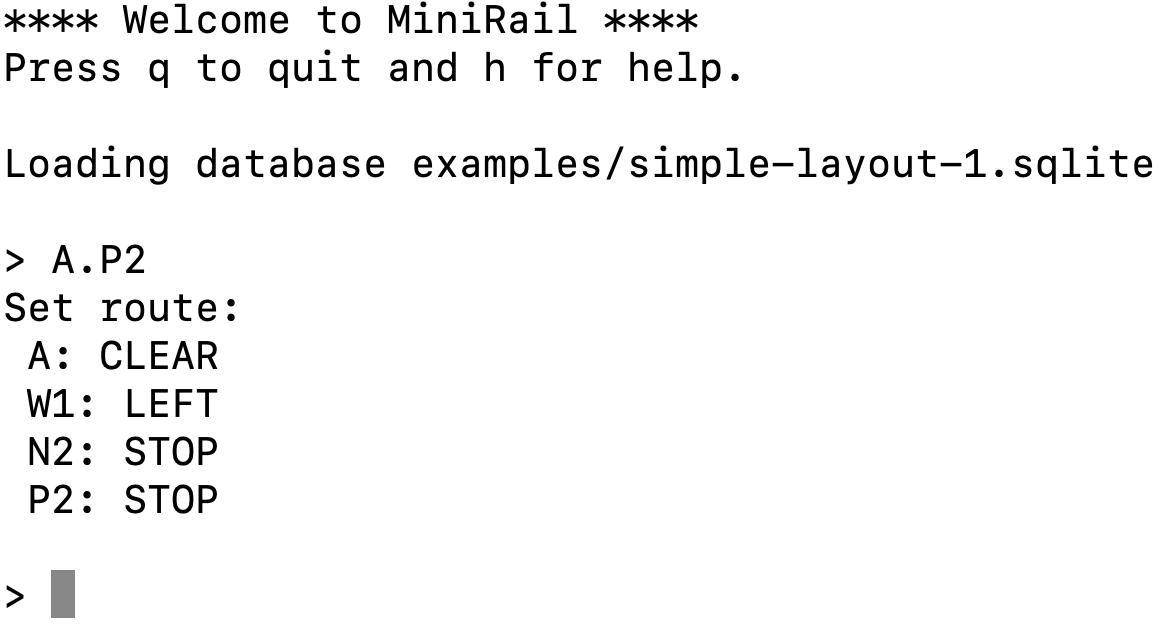
\includegraphics[width=.8\textwidth]{Assets/Images/5-Entwicklung-des-Stellwerks/Bedienung.png}
    \caption{Bedienoberfläche des Stellwerks}\label{abb:Entwicklung-des-Stellwerks:Bedienung}
\end{figure}

Die Topologie der Gleisanlage ist in einer SQLite-Datenbank gespeichert, welche beim Programmstart übergeben wird. Über einen \textit{Bedienstring} wird das Stellwerk gesteuert. Die Syntax ist hier immer \texttt{<start>.<ziel>} und hat das Stellen einer Zugfahrstraße von \texttt{start} nach \texttt{ziel} zur Folge.

Da die einzelnen Komponenten nicht miteinander kommunizieren können, handelt sich die Ausgabe um eine Simulation. Signale und Weichen werden also nicht wirklich gestellt.


\newpage
\section{Probleme bei der Kommunikation}\label{text:Entwicklung-des-Stellwerks:Probleme-bei-der-Kommunikation}

In \autoref{text:Methodik:Kommunikation} \nameref{text:Methodik:Kommunikation} wurde erläutert, wie die einzelnen Komponenten des Stellwerks miteinander kommunizieren können. Zunächst wurde ein CAN-Bus aufgebaut, der über eine USB-Brücke mit dem Computer über eine serielle Schnittstelle verbunden ist. Hierbei wurde beobachtet, der Bus an sich nur selten funktioniert. Das Fehlerbild beschränkt sich auf ein Volllaufen des Puffers beim Sendern einer Nachricht. Es wurde weiter festgestellt, dass der Fehler nicht deterministisch ist, da in manchen Fällen Daten gesendet und empfangen werden können.
Zu Testzwecken wurde der in \autoref{text:Methodik:Kommunikation:CAN-Bus} \nameref{text:Methodik:Kommunikation:CAN-Bus} dargestellte Testaufbau zweier Raspberry Pi Picos (\autoref{abb:Methodik:Kommunikation:CAN-Bus}) an die USB-Brücke angeschlossen. In seltenen Fällen gelang es, die Kommunikation beider Picos auf dem Computer mitzulesen. In der Regel stoppte der Bus, sobald man die Brücke angeschlossen hat.
Erst dann fiel auf, dass selbst jener Testaufbau nur selten funktioniert. Die Theorie, dass die Kontakte der Breadboards nicht sauber geschlossen werden, konnte weder bestätigt, noch widerlegt werden.

Als Notlösung wurde anschließend versucht, mit UART eine Art Bus zu simulieren (siehe \autoref{text:Methodik:Kommunikation:UART} \nameref{text:Methodik:Kommunikation:UART}). Hierbei kam es zu diversen Problemen, unter anderem dem Senden von Phantom-Bytes und der Kodierung empfangener Daten. Daher musste auch dieser Ansatz verworfen werden.


\chapter{Fazit und Ausblick}\label{text:Fazit-und-Ausblick}

In dieser Arbeit wurde die Entwicklung einer Gleisfreimeldeanlage und eines Stellwerks für eine Modelleisenbahn am Beispiel einer Klemmbausteineisenbahn durchgeführt. Nachdem in \autoref{text:Grundlagen} \nameref{text:Grundlagen} die Grundlagen der Eisenbahn, die Funktionsweise realer Stellwerke, sowie technische Grundlagen von Modelleisenbahnen erläutert wurden, führte \autoref{text:Methodik} \nameref{text:Methodik} aus, wie diese Konzepte auf eine Modelleisenbahn übertragen werden können. Im Anschluss wurden in \autoref{text:Entwicklung-der-GFA} \nameref{text:Entwicklung-der-GFA} sowie in \autoref{text:Entwicklung-des-Stellwerks} \nameref{text:Entwicklung-des-Stellwerks} die Implementierung einer Gleisfreimeldeanlage und eines Stellwerks in der Programmiersprache C beschrieben. \autoref{text:Auswertung} \nameref{text:Auswertung} hat die Ergebnisse ausgewertet und ist insbesondere auf Komplikationen eingegangen, die das Projekt letzten Endes scheitern ließen.

\section{Zusammenfassung}\label{text:Fazit-und-Ausblick:Zusammenfassung}

Es wurde gezeigt, dass die einzelnen entwickelten Komponenten funktionsfähig sind, jedoch lediglich deren Integration nicht umgesetzt werden konnte. Hier wäre es durch weiteres Experimentieren möglich, eine Lösung zu finden.

Bei einer erfolgreichen Umsetzung der Kommunikation zwischen den Komponenten lassen sich einige Folgeschritte ableiten:

\begin{description}
    \item[Decoder] Wie in \autoref{text:Entwicklung-des-Stellwerks:Signaldecoder} \nameref{text:Entwicklung-des-Stellwerks:Signaldecoder} und \autoref{text:Entwicklung-des-Stellwerks:Weichendecoder} \nameref{text:Entwicklung-des-Stellwerks:Weichendecoder} beschrieben, wurden die Decoder in dieser Arbeit nur konzeptuell behandelt. Für einen sinnvollen, realistischen Betrieb, müssen diese noch implementiert werden.
    \item[Verkabelung] In die Signale müssen kleine LEDs eingebaut werden und die Weichenantriebe müssen wie in \autoref{text:Entwicklung-des-Stellwerks:Weichendecoder} \nameref{text:Entwicklung-des-Stellwerks:Weichendecoder} beschrieben gebaut werden. Der Komplexität sind hier keine Grenzen gesetzt; so ist zum Beispiel die Entwicklung eigener Platinen möglich, um die Verkabelung zu vereinfachen.
    \item[Grafische Benutzeroberfläche] Zur Zeit kann das Stellwerk nur über die Kommandozeile bedient werden. Perspektivisch ist eine Bedienung analog zu einem realen \ac{ESTW} wünschenswert. Diese kann beispielsweise in C relativ einfach umgesetzt werden.
    \item[Zugsteuerung] Diese Arbeit hatte lediglich die Entwicklung eines Stellwerks nach realem Vorbild zum Ziel. Bei einer Modelleisenbahn ist aber oft auch eine Steuerung der Züge wünschenswert. Hierbei gibt es verschiedene Möglichkeiten, beispielsweise die vollständig manuelle Steuerung, oder eine vollautomatische Steuerung mit einem Decoder in jedem Zug über Funk oder Infrarot.
\end{description}

\section{Reflexion}\label{text:Fazit-und-Ausblick:Reflexion}

Diese Arbeit behandelte viele Aspekte, in denen die Autoren bisher wenig Erfahrung hatten. So stellte die Wahl der Programmiersprache C zu Beginn eine große Herausforderung dar. Aus moderneren Sprachen bekannte Wege mussten anders bestritten werden und nicht selten völlig anders gedacht werden. Die Nutzung von eingebetteten Systemen führte oft zu Problemen, da der Alltag in Vorlesungen oder auf der Arbeit sich fast ausschließlich auf klassische Computer-Architekturen beschränkt. Dies führte letztendlich auch dazu, dass die Kommunikation zwischen den Komponenten nicht mehr umgesetzt werden konnte.

Die Autoren nehmen aus diesem Projekte vor allem viele wertvolle Kenntnisse in der C-Programmierung und der Arbeit mit eingebetteten Systemen mit. Das Projekt motiviert zur Weiterentwicklung des Systems.



\clearpage
\cleardoublepage
\printbibliography

\printglossary[style=altlist, title=\labelGlossary]

\clearpage
\appendix
%!TEX root = ../Thesis.tex

\addchap{\labelAppendix}\label{appendix}

Anstelle eines Anhangs, kann der gesamte Quellcode auf GitHub gefunden werden: \href{https://github.com/yannickkirschen/study-project}{https://github.com/yannickkirschen/study-project}. Der eigentliche Code ist dabei im Unterverzeichnis \texttt{mini-rail}.

\end{document}
